\section{Casi d'uso}
I casi d'uso seguenti emergono da un'attenta analisi degli \textit{Analisti} del gruppo \GroupName{} rivolta al capitolato e da un'approfondita discussione con il proponente \Proponente{}. Gran parte dei casi d'uso sono stati dedotti grazie all'esperienza derivata dall'utilizzo di \glossario{ActiveAdmin}, un progetto analogo a \ProjectName{} basato su \glossario{Ruby on Rails}.\
Ogni caso d'uso è identificato univocamente e in modo gerarchico tramite una codifica nella forma:

\begin{center}

\textit{UC[codice dell'ambito][codice univoco del padre],[codice progressivo del figlio]}

\end{center} 

dove il \textbf{codice dell'ambito} può assumere i seguenti valori:

\begin{itemize}

  \item \textbf{U} - ambito utente, che comprende sia l'utente normale che l'\textit{admin} di una applicazione generata da \ProjectName{};
  \item \textbf{S} - ambito sviluppatore.
  \item \textbf{M} - ambito utente \glossario{MaaS} (MongoDB as an admin Service).

\end{itemize}
Per i tre ambiti(Utente,Sviluppatore,\glossario{MaaS}) il corrispondente diagramma delle 'Operazioni ad alto livello' è stato suddiviso per tipologia di utente, mantenendo per comodità la nomenclatura che ci sarebbe stata se non avessimo effettuato la suddivisione.
Nei diagrammi dei casi d'uso, il sistema dei livelli di astrazione inferiore si riferisce in modo ricorsivo al sistema del caso d'uso del padre. 
Per comodità di lettura viene utilizzato il nome del caso d'uso in analisi. 


\subsection{Ambito Utente}
\subsubsection{UCU - Operazioni ad alto livello - Utente non autenticato}    
    \begin{figure}[H]
      \begin{center}
      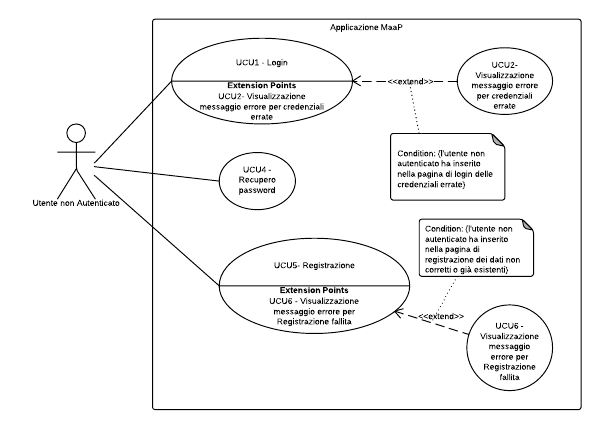
\includegraphics[scale=0.16]{UML/UCU - Operazioni ad alto livello - Utente non autenticato.png}
      \caption{UCU - Operazioni ad alto livello - Utente non autenticato}
      \end{center} 
    \end{figure}    
    
      %Tabella 
      \begin{center}
      \bgroup
      \def\arraystretch{1.8}     
      \begin{longtable}{  p{3.5cm} | p{8cm} } 
            
      \hline
      \multicolumn{2}{ | c | }{ \cellcolor[gray]{0.9} \textbf{UCU - Operazioni ad alto livello - Utente non autenticato}} \\ 
      \hline
      
      \textbf{Attori Primari} & Utente non autenticato  \\ 
          \textbf{Scopo e Descrizione} & L'Utente non autenticato può autenticarsi inserendo le credenziali nell'apposito form,può registrarsi all'applicazione se tale funzione è predisposta e può recuperare l'eventuale password d'accesso. \\ 
          
          \textbf{Precondizioni}  & L'applicazione MaaP è funzionante e pronta all'utilizzo.
Il sistema predispone all'utente non autenticato la pagina principale fornendo le funzionalità di autenticazione, registrazione e recupero password.\\ 
          
          \textbf{Postcondizioni} & L'applicazione ha ricevuto le informazioni sulle operazioni che l'utente vuole eseguire. \\ 
          \textbf{Flusso Principale} & 1. Utente non autenticato esegue il login (UCU1); \newline
2. Utente non autenticato può recuperare la password (UCU4); \newline
3. Utente non autenticato può richiedere la registrazione (UCU5); \newline \\
           \textbf{Estensioni} & 1.1 L'utente visualizza un messaggio di errore causato dall'inserimento di credenziali errate per il login (UCU2); \newline
3.1 L'utente a seguito del fallimento della registrazione, visualizza un messaggio di errore (UCU6). \\
      \end{longtable}
      \egroup
\end{center}

\subsubsection{UCU - Operazioni ad alto livello - Utente autenticato}    
    \begin{figure}[H]
      \begin{center}
      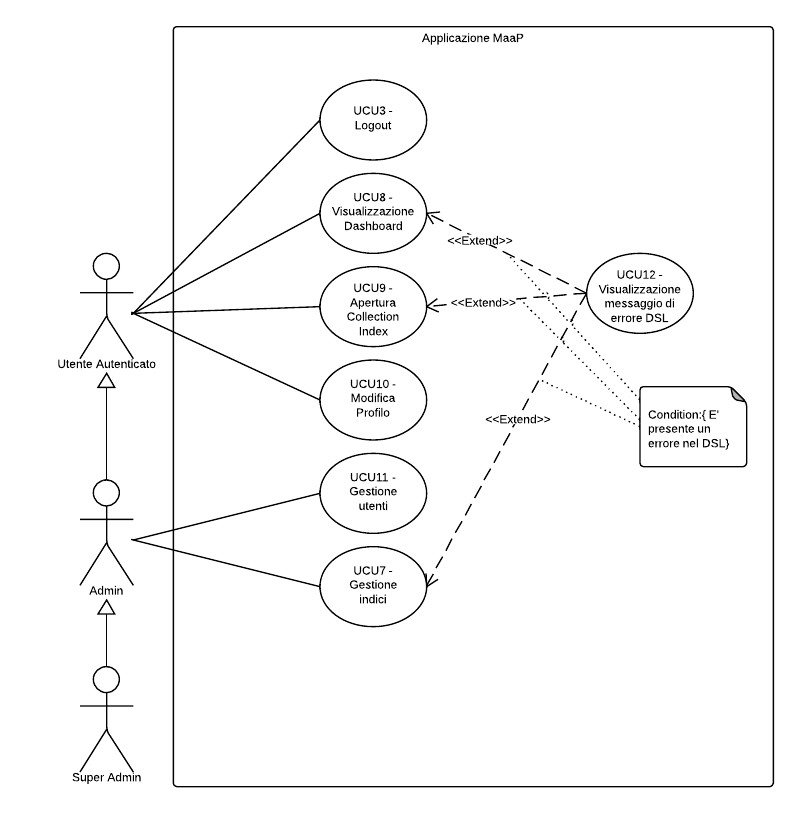
\includegraphics[scale=0.16]{UML/UCU - Operazioni ad alto livello - Utente autenticato.png}
      \caption{UCU - Operazioni ad alto livello - Utente autenticato}
      \end{center} 
    \end{figure}    
    
      %Tabella 
      \begin{center}
      \bgroup
      \def\arraystretch{1.8}     
      \begin{longtable}{  p{3.5cm} | p{8cm} } 
            
      \hline
      \multicolumn{2}{ | c | }{ \cellcolor[gray]{0.9} \textbf{UCU - Operazioni ad alto livello - Utente autenticato}} \\ 
      \hline
      
      \textbf{Attori Primari} & Utente autenticato, Admin \\ 
          \textbf{Scopo e Descrizione} & L'Utente autenticato in qualsiasi punto dell'applicazione può accedere alle seguenti funzionalità: accedere alla Dashboard, effettuare il Logout , può scegliere una qualsiasi collection presente e può modificare i propri dati. 
L'Utente Admin eredita le funzionalità dell'Utente Autenticato, può gestire gli utenti creandone di nuovi o modificandoli ed inoltre può gestire nuovi indici. \\ 
          
          \textbf{Precondizioni}  & L'applicazione MaaP è funzionante e pronta all'utilizzo.
Il sistema predispone all'utente autenticato la corrispondente pagina dashboard.\\ 
          
          \textbf{Postcondizioni} & L'applicazione ha ricevuto le informazioni sulle operazioni che l'utente autenticato vuole eseguire. \\ 
          \textbf{Flusso Principale} & 1. L'utente autenticato può decidere di effettuare il logout (UCU3); \newline
2. L'utente autenticato può visualizzare la Dashboard (UCU8); \newline
3. L'utente autenticato può scegliere una collection e visualizzarla (UCU9); \newline
4. L'utente autenticato può scegliere di modificare i propri dati (UCU10); \newline
5. L'admin può accede alla sua pagina di amministrazione per la gestione degli utenti (UCU11); \newline
6. L'admin può gestire i possibili indici (UCU7). \newline
 \\
           \textbf{Estensioni} & 2.1. L'utente visualizza un messaggio di errore dovuto al rilevamento da parte dell'applicazione di un errore causato da un file scritto con il DSL invece della pagina di \glossario{dashboard}(UCU12); \newline
3.1.  L'utente visualizza un messaggio di errore dovuto al rilevamento da parte dell'applicazione di un errore causato da un file scritto con il DSL invece della \glossario{collection} selezionata (UCU12); \newline
6.1.  L'admin visualizza un messaggio di errore dovuto al rilevamento da parte dell'applicazione di un errore causato da un file scritto con il DSL invece della pagina di gestione degli indici (UCU12). \\
      \end{longtable}
      \egroup
\end{center}

\subsubsection{UCU1 - Login}    
    \begin{figure}[H]
      \begin{center}
      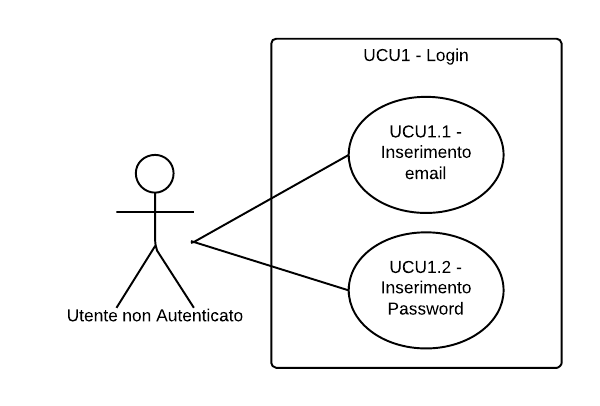
\includegraphics[scale=0.16]{UML/UCU1 - Login.png}
      \caption{UCU1 - Login}
      \end{center} 
    \end{figure}    
    
      %Tabella 
      \begin{center}
      \bgroup
      \def\arraystretch{1.8}     
      \begin{longtable}{  p{3.5cm} | p{8cm} } 
            
      \hline
      \multicolumn{2}{ | c | }{ \cellcolor[gray]{0.9} \textbf{UCU1 - Login}} \\ 
      \hline
      
      \textbf{Attori Primari} & Utente non autenticato  \\ 
          \textbf{Scopo e Descrizione} & L'utente non autenticato intende accedere all'applicazione, per farlo deve inserire le proprie credenziali composte da una email ed una password.  \\ 
          
          \textbf{Precondizioni}  & L'applicazione predispone la pagina di autenticazione all'utente non autenticato fornendo un apposito form per l'inserimento delle credenziali.\\ 
          
          \textbf{Postcondizioni} & Il sistema ha autenticato l'utente e lo ha rediretto alla pagina Dashboard. \\ 
          \textbf{Flusso Principale} & 1. L'utente inserisce l'email (UC1.1); \newline
2. L'utente inserisce la password (UC1.2). \newline \\
           \textbf{Scenari Alternativi} & 1. L'utente non effettua l'autenticazione. \\
      \end{longtable}
      \egroup
\end{center}

\subsubsection{UCU1.1 - Inserimento email} 
      %Tabella 
      \begin{center}
      \bgroup
      \def\arraystretch{1.8}     
      \begin{longtable}{  p{3.5cm} | p{8cm} } 
            
      \hline
      \multicolumn{2}{ | c | }{ \cellcolor[gray]{0.9} \textbf{UCU1.1 - Inserimento email}} \\ 
      \hline
      
      \textbf{Attori Primari} & Utente non autenticato  \\ 
          \textbf{Scopo e Descrizione} & L'utente non autenticato inserisce l'email con la quale è registrato all'applicazione. \\ 
          
          \textbf{Precondizioni}  & L'applicazione  /glossario{Maap} è pronta e l'utente intende autenticarsi.\\ 
          
          \textbf{Postcondizioni} & L'applicazione ha l'informazione relativa all'email inserita dall'utente. \\ 
          \textbf{Flusso Principale} & 1. L'utente non autenticato inserisce la propria email per procedere con l'autenticazione (UCU1.1). \\
          
      \end{longtable}
      \egroup
\end{center}

\subsubsection{UCU1.2 - Inserimento Password} 
      %Tabella 
      \begin{center}
      \bgroup
      \def\arraystretch{1.8}     
      \begin{longtable}{  p{3.5cm} | p{8cm} } 
            
      \hline
      \multicolumn{2}{ | c | }{ \cellcolor[gray]{0.9} \textbf{UCU1.2 - Inserimento Password}} \\ 
      \hline
      
      \textbf{Attori Primari} & Utente non autenticato  \\ 
          \textbf{Scopo e Descrizione} & L'utente non autenticato inserisce la password per effettuare l'autenticazione.
Tale password dovrà essere alfanumerica e con una lunghezza minima di 8 caratteri. \\ 
          
          \textbf{Precondizioni}  & L'applicazione  /glossario{MaaP} è pronta e l'utente intende autenticarsi.\\ 
          
          \textbf{Postcondizioni} & L'applicazione ha l'informazione relativa alla password inserita dall'utente. \\ 
          \textbf{Flusso Principale} & 1. L'utente non autenticato inserisce la propria password di accesso all'applicazione  /glossario{MaaP} (UCU1.2). \\
          
      \end{longtable}
      \egroup
\end{center}

\subsubsection{UCU2 - Visualizzazione messaggio errore per credenziali errate} 
      %Tabella 
      \begin{center}
      \bgroup
      \def\arraystretch{1.8}     
      \begin{longtable}{  p{3.5cm} | p{8cm} } 
            
      \hline
      \multicolumn{2}{ | c | }{ \cellcolor[gray]{0.9} \textbf{UCU2 - Visualizzazione messaggio errore per credenziali errate}} \\ 
      \hline
      
      \textbf{Attori Primari} & Utente non autenticato  \\ 
          \textbf{Scopo e Descrizione} & L'utente visualizza un messaggio di errore dato dall'inserimento di credenziali errate. \\ 
          
          \textbf{Precondizioni}  & L'applicazione ha verificato le credenziali inserite dall'utente.\\ 
          
          \textbf{Postcondizioni} & L'applicazione predispone la visualizzazione di un messaggio di errore e non autentica l'utente al sistema. \\ 
          \textbf{Flusso Principale} & 1. L'utente non autenticato a seguito del tentativo di effettuare il login visualizza un messaggio di errore dato dal fallimento dell'operazione (UCU2). \\
          
      \end{longtable}
      \egroup
\end{center}

\subsubsection{UCU3 - Logout} 
      %Tabella 
      \begin{center}
      \bgroup
      \def\arraystretch{1.8}     
      \begin{longtable}{  p{3.5cm} | p{8cm} } 
            
      \hline
      \multicolumn{2}{ | c | }{ \cellcolor[gray]{0.9} \textbf{UCU3 - Logout}} \\ 
      \hline
      
      \textbf{Attori Primari} & Utente autenticato, Admin \\ 
          \textbf{Scopo e Descrizione} & L'utente autenticato può eseguire il logout dall'applicazione. \\ 
          
          \textbf{Precondizioni}  & L'applicazione ha una sessione attiva dell'utente autenticato e mette a disposizione a quest'ultimo la possibilità di effettuare il logout.\\ 
          
          \textbf{Postcondizioni} & L'applicazione ha eseguito il logout richiesto dall'utente chiudendo la sessione di quest'ultimo. \\ 
          \textbf{Flusso Principale} & 1. L'utente seleziona il logout (UCU3).  \\
          
      \end{longtable}
      \egroup
\end{center}

\subsubsection{UCU4 - Recupero password}    
    \begin{figure}[H]
      \begin{center}
      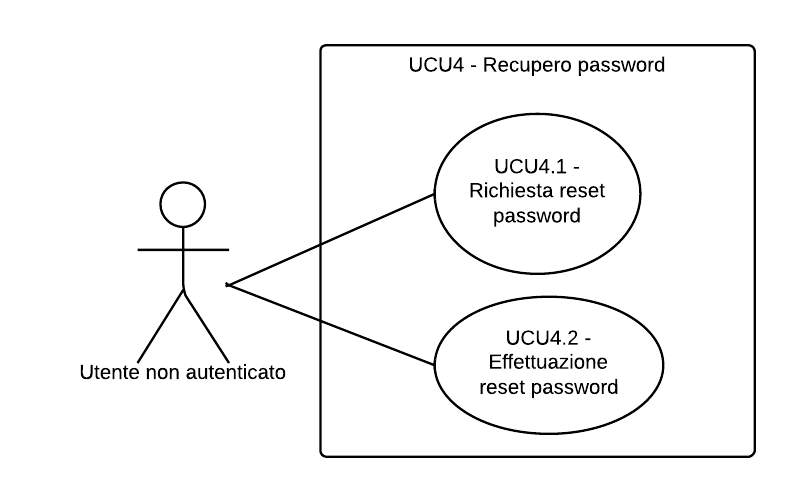
\includegraphics[scale=0.16]{UML/UCU4 - Recupero password.png}
      \caption{UCU4 - Recupero password}
      \end{center} 
    \end{figure}    
    
      %Tabella 
      \begin{center}
      \bgroup
      \def\arraystretch{1.8}     
      \begin{longtable}{  p{3.5cm} | p{8cm} } 
            
      \hline
      \multicolumn{2}{ | c | }{ \cellcolor[gray]{0.9} \textbf{UCU4 - Recupero password}} \\ 
      \hline
      
      \textbf{Attori Primari} & Utente non autenticato  \\ 
          \textbf{Scopo e Descrizione} & L'utente intende recuperare la password d'accesso all'applicazione. \\ 
          
          \textbf{Precondizioni}  & L'applicazione predispone e mostra all'utente non autenticato la possibilità di recupero password.\\ 
          
          \textbf{Postcondizioni} & L'applicazione ha effettuato le operazioni necessarie per il recupero password richiesta dall'utente non autenticato. \\ 
          \textbf{Flusso Principale} & 1. L'utente richiede il reset della propria password d'accesso all'applicazione (UCU4.1);
2. L'utente, il quale ha richiesto reset della password, attraverso un link contenuto nell'email inviata dal sistema, accede alla pagina per il reset della password (UCU4.2). \\
          
      \end{longtable}
      \egroup
\end{center}

\subsubsection{UCU4.1 - Richiesta reset password}    
    \begin{figure}[H]
      \begin{center}
      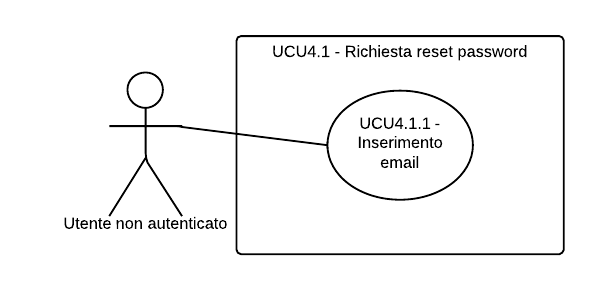
\includegraphics[scale=0.16]{UML/UCU4.1 - Richiesta reset password.png}
      \caption{UCU4.1 - Richiesta reset password}
      \end{center} 
    \end{figure}    
    
      %Tabella 
      \begin{center}
      \bgroup
      \def\arraystretch{1.8}     
      \begin{longtable}{  p{3.5cm} | p{8cm} } 
            
      \hline
      \multicolumn{2}{ | c | }{ \cellcolor[gray]{0.9} \textbf{UCU4.1 - Richiesta reset password}} \\ 
      \hline
      
      \textbf{Attori Primari} & Utente non autenticato \\ 
          \textbf{Scopo e Descrizione} & L'utente intende richiedere il reset della propria password d'accesso all'applicazione, per poterlo fare dovrà inserire un indirizzo email nel quale verrà inviata un email contenente il link dal quale potrà accedere alla pagina per effettuare il reset della propria password. \\ 
          
          \textbf{Precondizioni}  & Il sistema predispone all'utente non autenticato una pagina con rispettivo modulo di inserimento dell'email per portare a termine la procedura di reset della password.\\ 
          
          \textbf{Postcondizioni} & Il sistema ha inviato correttamente l'email contente il link per completare la procedura relativa al reset della password utente. \\ 
          \textbf{Flusso Principale} & 1. L'utente inserisce una email su cui verrà inviata l'email per completare l'operazione di reset della password (UCU4.1.1). \\
          
      \end{longtable}
      \egroup
\end{center}

\subsubsection{UCU4.1.1 - Inserimento email} 
      %Tabella 
      \begin{center}
      \bgroup
      \def\arraystretch{1.8}     
      \begin{longtable}{  p{3.5cm} | p{8cm} } 
            
      \hline
      \multicolumn{2}{ | c | }{ \cellcolor[gray]{0.9} \textbf{UCU4.1.1 - Inserimento email}} \\ 
      \hline
      
      \textbf{Attori Primari} & Utente non autenticato  \\ 
          \textbf{Scopo e Descrizione} & L'utente non autenticato intende inserire l'email per procedere con il recupero della propria password per l'accesso all'applicazione. \\ 
          
          \textbf{Precondizioni}  & L'applicazione predispone la pagina per il reset password mostrando il relativo modulo per l'inserimento dell'email ed è pronta per l'iterazione dell'utente.\\ 
          
          \textbf{Postcondizioni} & L'applicazione ha ricevuto il dato relativo all'email inserita dall'utente ed ha effettuato l'invio dell'email con link per il completamento dell'operazione di reset. \\ 
          \textbf{Flusso Principale} & 1. L'utente inserisce l'email per il recupero della password di accesso (UCU4.1.1). \\
          
      \end{longtable}
      \egroup
\end{center}

\subsubsection{UCU4.2 - Effettuazione reset password}    
    \begin{figure}[H]
      \begin{center}
      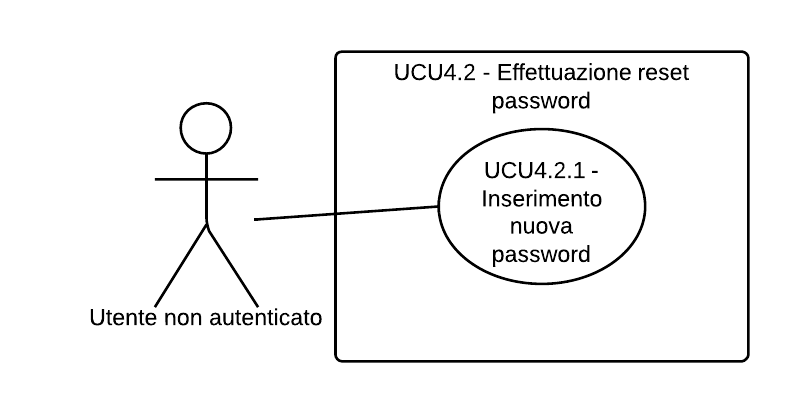
\includegraphics[scale=0.16]{UML/UCU4.2 - Effettuazione reset password.png}
      \caption{UCU4.2 - Effettuazione reset password}
      \end{center} 
    \end{figure}    
    
      %Tabella 
      \begin{center}
      \bgroup
      \def\arraystretch{1.8}     
      \begin{longtable}{  p{3.5cm} | p{8cm} } 
            
      \hline
      \multicolumn{2}{ | c | }{ \cellcolor[gray]{0.9} \textbf{UCU4.2 - Effettuazione reset password}} \\ 
      \hline
      
      \textbf{Attori Primari} & Utente non autenticato  \\ 
          \textbf{Scopo e Descrizione} & L'utente intende una nuova password che sostituirà quella precedente per l'accesso all'applicazione.
La password deve essere alfanumerica e con lunghezza minima 8 caratteri. \\ 
          
          \textbf{Precondizioni}  & Il sistema ha inviato all'utente non autenticato un'email contenente il link della pagina corrente visualizzata.\\ 
          
          \textbf{Postcondizioni} & Il sistema ha effettuato il reset della password dell'utente con il dato della nuova password inserito da quest'ultimo. \\ 
          \textbf{Flusso Principale} & 1. L'utente inserisce la nuova password (UCU4.2.1). \\
           \textbf{Scenari Alternativi} & 1.  L'utente può Inserire la nuova password con la quale intende accede all'applicazione (UCU4.2.1). \\
      \end{longtable}
      \egroup
\end{center}

\subsubsection{UCU4.2.1 - Inserimento nuova password} 
      %Tabella 
      \begin{center}
      \bgroup
      \def\arraystretch{1.8}     
      \begin{longtable}{  p{3.5cm} | p{8cm} } 
            
      \hline
      \multicolumn{2}{ | c | }{ \cellcolor[gray]{0.9} \textbf{UCU4.2.1 - Inserimento nuova password}} \\ 
      \hline
      
      \textbf{Attori Primari} & Utente non autenticato  \\ 
          \textbf{Scopo e Descrizione} & L'utente desidera inserire una nuova password che sostituisca la precedente password perduta per poter accede all'applicazione.
La nuova password che l'utente deve inserire deve essere alfanumerica di minimo 8 caratteri. \\ 
          
          \textbf{Precondizioni}  & Il sistema ha inviato un'email contenente il link della pagina correntemente visualizzata dall'utente non autenticato e predispone un form per l'inserimento della nuova password.\\ 
          
          \textbf{Postcondizioni} & Il sistema ha ricevuto il dato relativo alla nuova password di accesso del corrispondente utente. \\ 
          \textbf{Flusso Principale} & 1. L'utente inserisce la nuova password che sostituisce la precedente come password d'accesso all'applicazione (UCU4.2.1). \\
          
      \end{longtable}
      \egroup
\end{center}

\subsubsection{UCU5 - Registrazione}    
    \begin{figure}[H]
      \begin{center}
      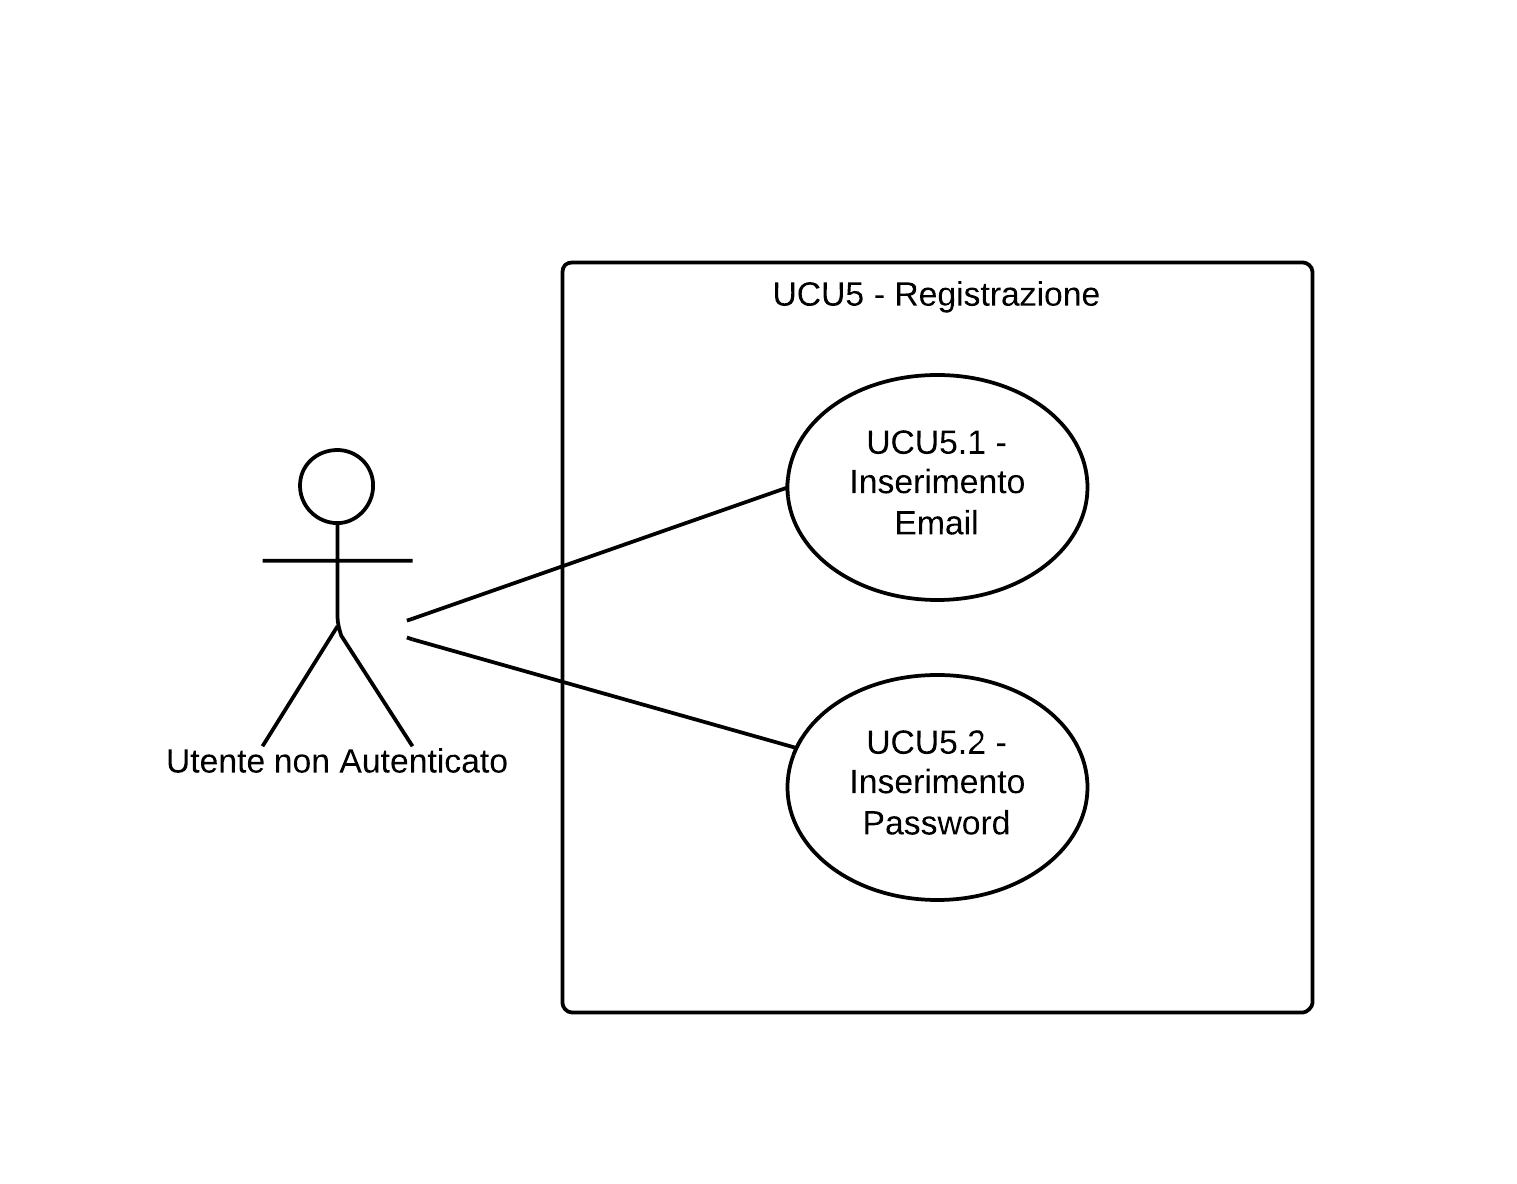
\includegraphics[scale=0.16]{UML/UCU5 - Registrazione.png}
      \caption{UCU5 - Registrazione}
      \end{center} 
    \end{figure}    
    
      %Tabella 
      \begin{center}
      \bgroup
      \def\arraystretch{1.8}     
      \begin{longtable}{  p{3.5cm} | p{8cm} } 
            
      \hline
      \multicolumn{2}{ | c | }{ \cellcolor[gray]{0.9} \textbf{UCU5 - Registrazione}} \\ 
      \hline
      
      \textbf{Attori Primari} & Utente non autenticato  \\ 
          \textbf{Scopo e Descrizione} & L'utente intende registrarsi all'applicazione e per farlo deve inserire negli appositi campi email e password. \\ 
          
          \textbf{Precondizioni}  & L'applicazione predispone la possibilità di registrazione.\\ 
          
          \textbf{Postcondizioni} & L'applicazione ha creato un nuovo account utente assegnandogli di default il livello "utente". \\ 
          \textbf{Flusso Principale} & 1. L'utente non autenticato inserisce l'email (UCU5.1);  \newline
2. L'utente non autenticato inserisce la password (UCU5.2). \\
           \textbf{Scenari Alternativi} & 1. L'utente non autenticato interrompe l'operazione di registrazione non creando un nuovo account. \\
      \end{longtable}
      \egroup
\end{center}

\subsubsection{UCU6 - Visualizzazione messaggio errore per Registrazione fallita} 
      %Tabella 
      \begin{center}
      \bgroup
      \def\arraystretch{1.8}     
      \begin{longtable}{  p{3.5cm} | p{8cm} } 
            
      \hline
      \multicolumn{2}{ | c | }{ \cellcolor[gray]{0.9} \textbf{UCU6 - Visualizzazione messaggio errore per Registrazione fallita}} \\ 
      \hline
      
      \textbf{Attori Primari} & Utente non autenticato  \\ 
          \textbf{Scopo e Descrizione} & L'applicazione visualizza un messaggio d'errore all'utente causata dall'inserimento di credenziali non corrette o già presenti nel database. \\ 
          
          \textbf{Precondizioni}  & L'applicazione ha ricevuto i dati di registrazione inseriti dall'utente non autenticato e tenta la creazione di un nuovo account.\\ 
          
          \textbf{Postcondizioni} & L'applicazione mostra un messaggio di errore dato dal fallimento del tentativo di registrazione richiesta dall'utente non autenticato. \\ 
          \textbf{Flusso Principale} & 1. L'utente non autenticato ha tentato di registrarsi all'applicazione con risultato il fallimento dell'operazione e la visualizzazione di un messaggio di errore (UCU6). \\
          
      \end{longtable}
      \egroup
\end{center}

\subsubsection{UCU7 - Gestione indici}    
    \begin{figure}[H]
      \begin{center}
      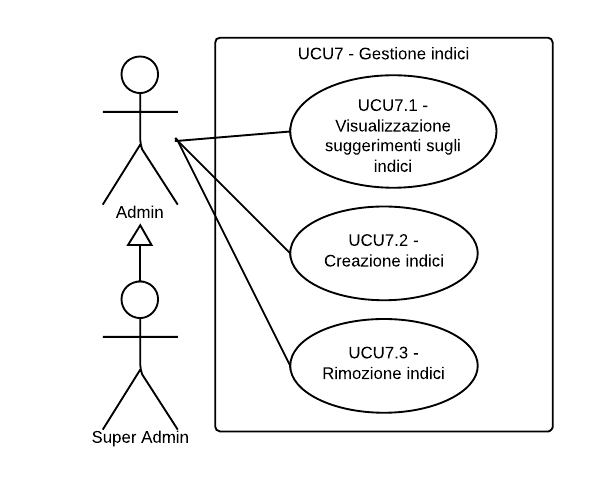
\includegraphics[scale=0.16]{UML/UCU7 - Gestione indici.png}
      \caption{UCU7 - Gestione indici}
      \end{center} 
    \end{figure}    
    
      %Tabella 
      \begin{center}
      \bgroup
      \def\arraystretch{1.8}     
      \begin{longtable}{  p{3.5cm} | p{8cm} } 
            
      \hline
      \multicolumn{2}{ | c | }{ \cellcolor[gray]{0.9} \textbf{UCU7 - Gestione indici}} \\ 
      \hline
      
      \textbf{Attori Primari} & Admin \\ 
          \textbf{Scopo e Descrizione} & L'admin può visualizzare i suggerimenti proposti sugli indici e può decidere di aggiungerli.  \newline
Gli indici già presenti possono essere eliminati. \\ 
          
          \textbf{Precondizioni}  & L'applicazione mette a disposizione dell'admin la pagina per gestire gli indici sulla base delle query più utilizzate.\\ 
          
          \textbf{Postcondizioni} & L'applicazione ha creato gli indici selezionati dall'admin. \\ 
          \textbf{Flusso Principale} & 1. La pagina di gestione visualizza i suggerimenti per la creazione degli indici (UCU7.1);  \newline
2. La pagina di gestione permette all'admin la creazione degli indici suggeriti (UCU7.2);  \newline
3. La pagina di gestione permette all'admin l'eliminazione degli indici suggeriti (UCU7.2).  \newline \\
          
      \end{longtable}
      \egroup
\end{center}

\subsubsection{UCU7.1 - Visualizzazione suggerimenti sugli indici} 
      %Tabella 
      \begin{center}
      \bgroup
      \def\arraystretch{1.8}     
      \begin{longtable}{  p{3.5cm} | p{8cm} } 
            
      \hline
      \multicolumn{2}{ | c | }{ \cellcolor[gray]{0.9} \textbf{UCU7.1 - Visualizzazione suggerimenti sugli indici}} \\ 
      \hline
      
      \textbf{Attori Primari} & Admin \\ 
          \textbf{Scopo e Descrizione} & La pagina di gestione degli indici fornisce all'admin un elenco suggerito di attributi a cui applicare gli indici in base alle query più utilizzate. \\ 
          
          \textbf{Precondizioni}  & L'applicazione ha eseguito una ricerca sulla base delle query più utilizzate. \\ 
          
          \textbf{Postcondizioni} & L'applicazione visualizza correttamente tutti i suggerimenti derivati dalla ricerca. \\ 
          \textbf{Flusso Principale} & 1. L'admin visualizza una serie di indici suggeriti dall'applicazione (UCU7.1). \\
          
      \end{longtable}
      \egroup
\end{center}

\subsubsection{UCU7.2 - Creazione indici} 
      %Tabella 
      \begin{center}
      \bgroup
      \def\arraystretch{1.8}     
      \begin{longtable}{  p{3.5cm} | p{8cm} } 
            
      \hline
      \multicolumn{2}{ | c | }{ \cellcolor[gray]{0.9} \textbf{UCU7.2 - Creazione indici}} \\ 
      \hline
      
      \textbf{Attori Primari} & Admin \\ 
          \textbf{Scopo e Descrizione} & L'Admin seleziona gli indici suggeriti e li crea. \\ 
          
          \textbf{Precondizioni}  & L'applicazione visualizza correttamente la lista degli indici suggeriti.\\ 
          
          \textbf{Postcondizioni} & L'applicazione ha creato gli indici selezionati dall'Admin. \\ 
          \textbf{Flusso Principale} & 1. L'admin seleziona e crea indici tra quelli disponibili suggeriti dall'applicazione (UCU7.2). \\
          
      \end{longtable}
      \egroup
\end{center}

\subsubsection{UCU7.3 - Rimozione indici} 
      %Tabella 
      \begin{center}
      \bgroup
      \def\arraystretch{1.8}     
      \begin{longtable}{  p{3.5cm} | p{8cm} } 
            
      \hline
      \multicolumn{2}{ | c | }{ \cellcolor[gray]{0.9} \textbf{UCU7.3 - Rimozione indici}} \\ 
      \hline
      
      \textbf{Attori Primari} & Admin \\ 
          \textbf{Scopo e Descrizione} & L'Admin seleziona gli indici visualizzati dall'applicazione e li rimuove. \\ 
          
          \textbf{Precondizioni}  & L'applicazione visualizza correttamente la lista degli indici.\\ 
          
          \textbf{Postcondizioni} & L'applicazione ha eliminato gli indici selezionati dall'Admin. \\ 
          \textbf{Flusso Principale} & 1. L'admin seleziona e rimuove indici dalla lista di quelli presenti (UCU7.3). \\
          
      \end{longtable}
      \egroup
\end{center}

\subsubsection{UCU8 - Visualizzazione Dashboard} 
      %Tabella 
      \begin{center}
      \bgroup
      \def\arraystretch{1.8}     
      \begin{longtable}{  p{3.5cm} | p{8cm} } 
            
      \hline
      \multicolumn{2}{ | c | }{ \cellcolor[gray]{0.9} \textbf{UCU8 - Visualizzazione Dashboard}} \\ 
      \hline
      
      \textbf{Attori Primari} & Utente autenticato, Admin \\ 
          \textbf{Scopo e Descrizione} & L'utente autenticato può visualizzare la pagina di Dashboard nella quale potrà aver accesso ad esempio alla lista delle collection presenti e ad altre funzionalità disponibili. \\ 
          
          \textbf{Precondizioni}  & L'applicazione predispone la pagina di Dashboard all'utente autenticato.\\ 
          
          \textbf{Postcondizioni} & L'applicazione visualizza all'utente la pagina di Dashboard ed pronta ad interagire con l'utente per svolgere le operazioni che desidera eseguire.
 \\ 
          \textbf{Flusso Principale} & 1. L'utente autenticato visualizza la propria Dashboard (UCU8). \\
          
      \end{longtable}
      \egroup
\end{center}

\subsubsection{UCU9 - Apertura Collection Index}    
    \begin{figure}[H]
      \begin{center}
      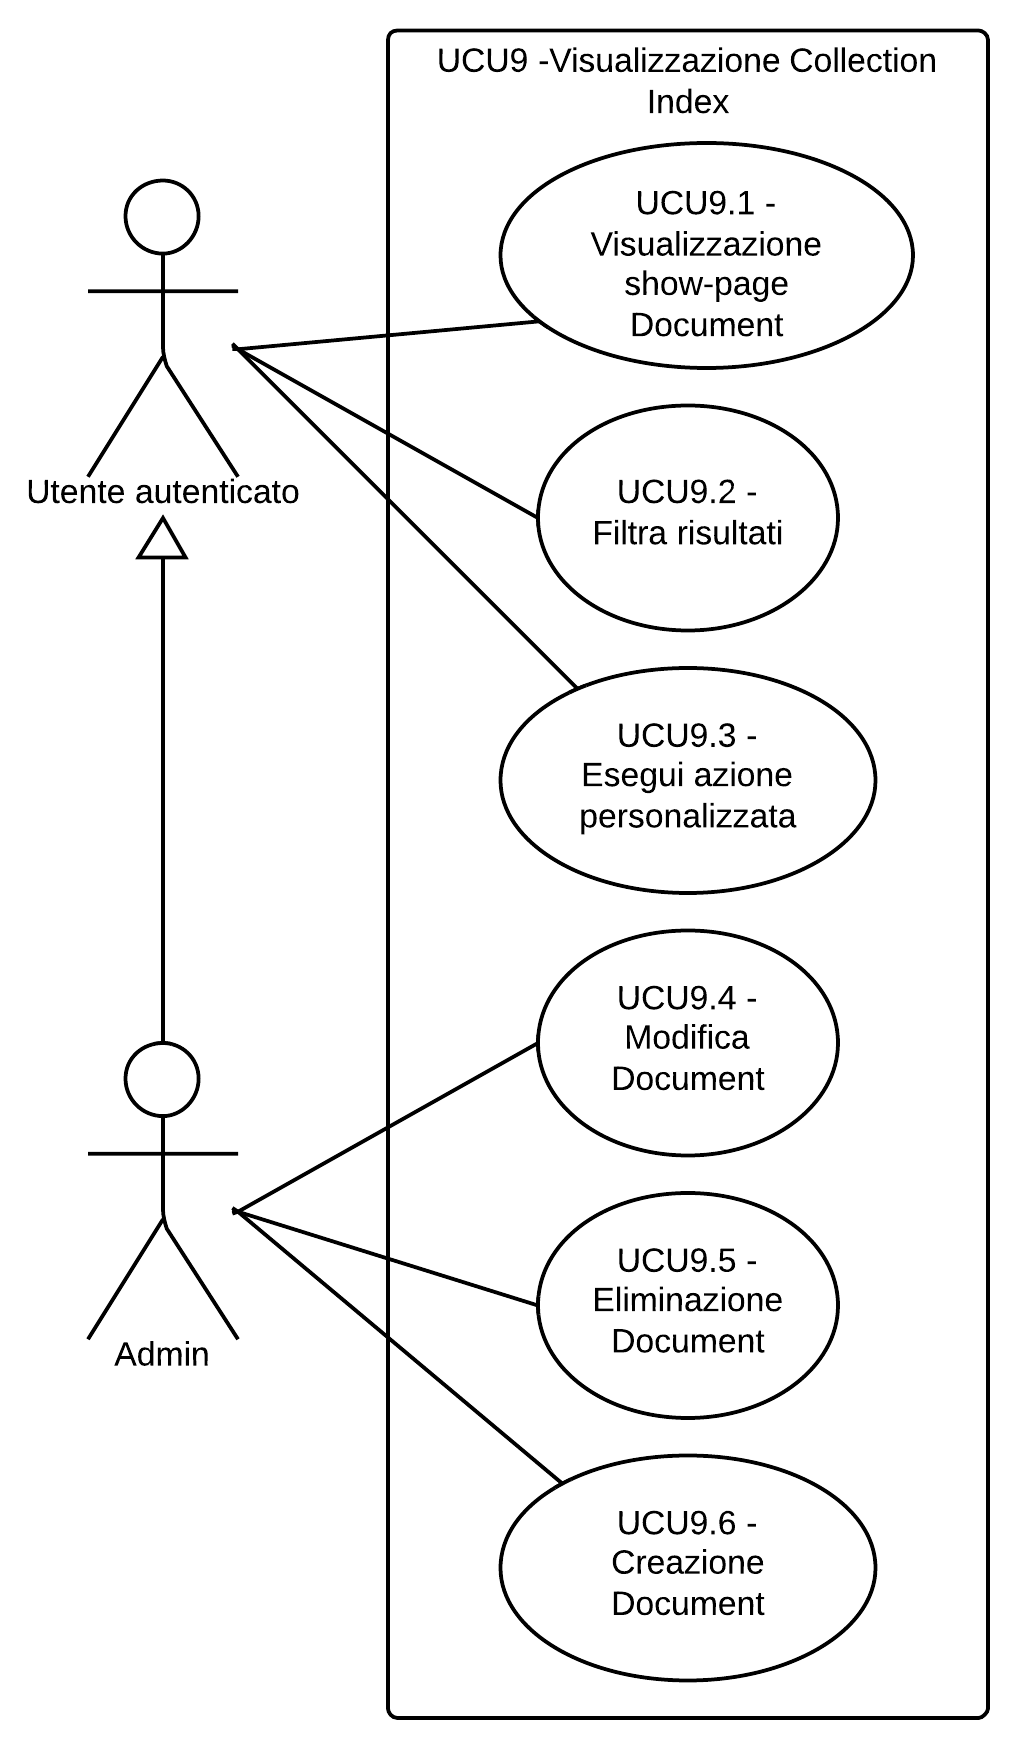
\includegraphics[scale=0.16]{UML/UCU9 - Apertura Collection Index.png}
      \caption{UCU9 - Apertura Collection Index}
      \end{center} 
    \end{figure}    
    
      %Tabella 
      \begin{center}
      \bgroup
      \def\arraystretch{1.8}     
      \begin{longtable}{  p{3.5cm} | p{8cm} } 
            
      \hline
      \multicolumn{2}{ | c | }{ \cellcolor[gray]{0.9} \textbf{UCU9 - Apertura Collection Index}} \\ 
      \hline
      
      \textbf{Attori Primari} & Utente autenticato, Admin \\ 
          \textbf{Scopo e Descrizione} & L'utente autenticato, selezionata una \glossario{Collection}, ne visualizza in forma tabellare tutti i documenti che contiene.  \newline
Di questa collection può filtrarne i risultati visualizzabili, può eseguire tramite bottoni predisposti nella pagina azioni personalizzati e per ogni \glossario{Document}, selezionarlo e visualizzarne la show-page corrispondente.  \newline
L'Admin ha i permessi per modificare un documento o eliminare un \glossario{Document}.  \newline \\ 
          
          \textbf{Precondizioni}  & L'applicazione ha ricevuto la richiesta da parte dell'utente autenticato di visualizzare la \glossario{Collection}.\\ 
          
          \textbf{Postcondizioni} & L'applicazione ha visualizzato la \glossario{Collection-Index} ed ha recepito le informazioni sulle operazioni che l'utente desidera eseguire. \\ 
          \textbf{Flusso Principale} & 1. L'utente autenticato può aprire la show-page relativa ad un \glossario{Document} (UCU9.1);  \newline
2. L'utente autenticato può filtrare la  \glossario{Collection} (UCU9.2);  \newline
3. L'utente autenticato può eseguire un'azione personalizzata se è presente (UCU9.3);  \newline
4. L'Admin può modificare un \glossario{Document} (UCU9.4);  \newline
5. L'Admin può eliminare un \glossario{Document} (UCU9.5).  \newline \\
           \textbf{Estensioni} & 4.1 L'admin annulla la modifica Document (UCU9.7). \\
      \end{longtable}
      \egroup
\end{center}

\subsubsection{UCU9.1 - Apertura show-page Document}    
    \begin{figure}[H]
      \begin{center}
      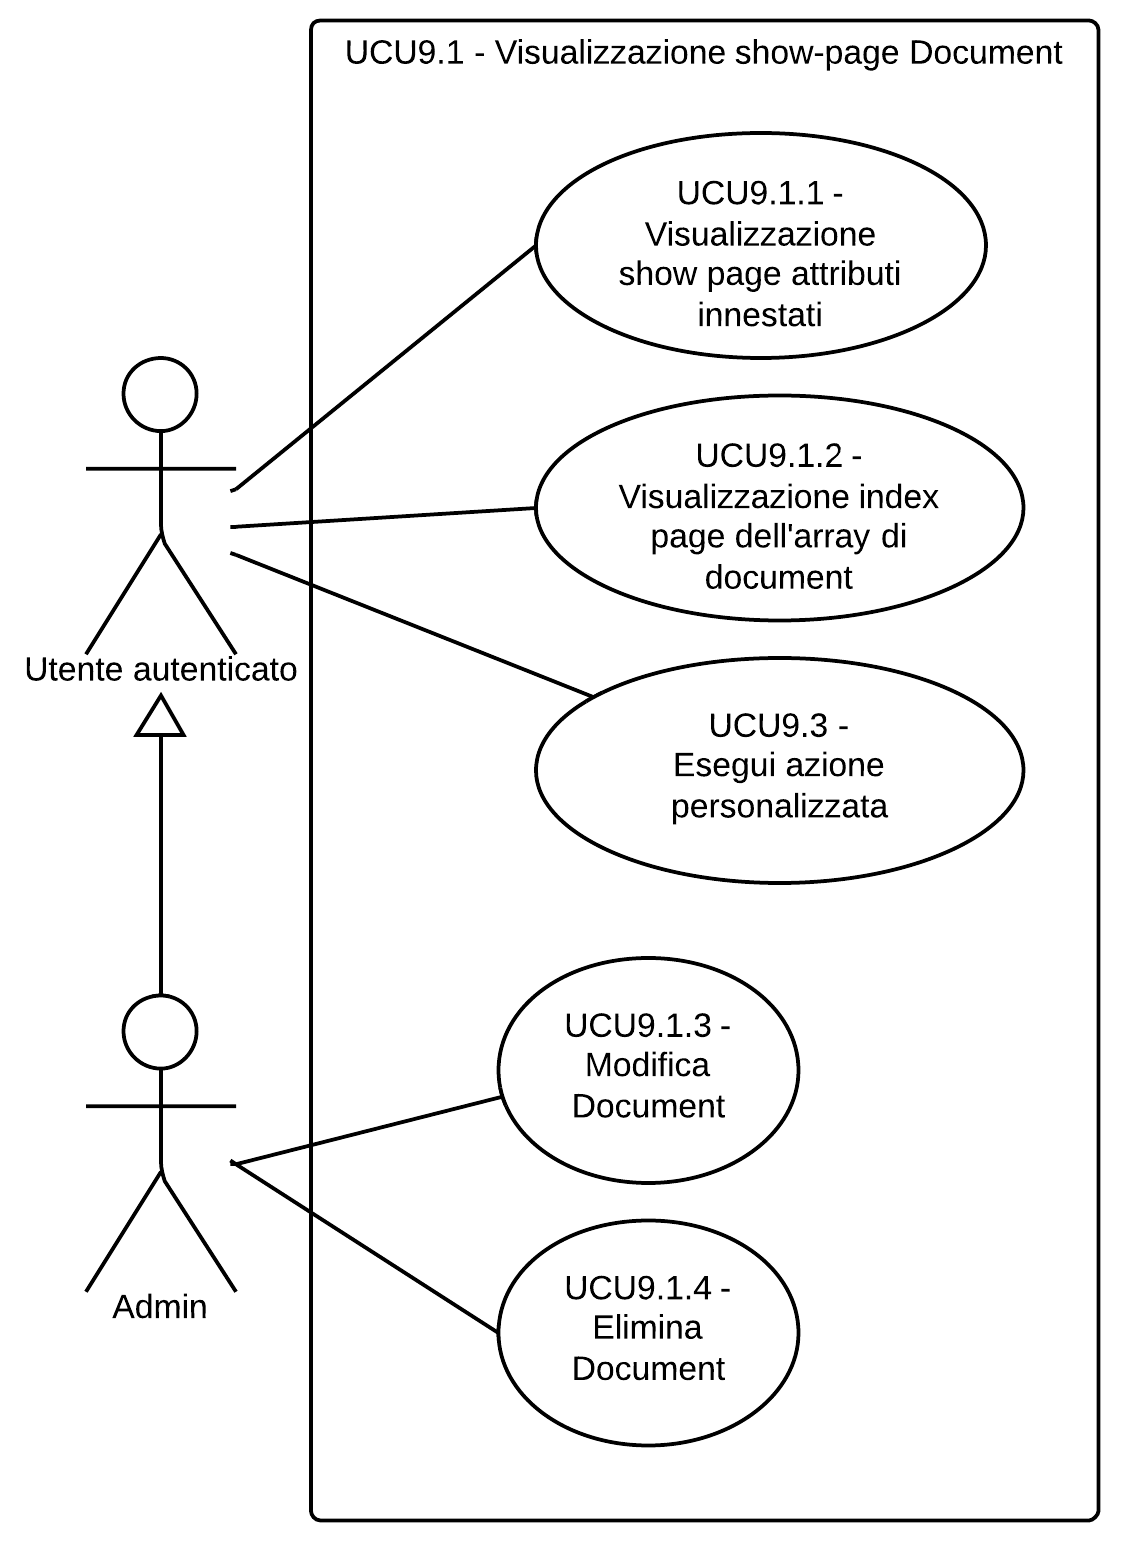
\includegraphics[scale=0.16]{UML/UCU9.1 - Apertura show-page Document.png}
      \caption{UCU9.1 - Apertura show-page Document}
      \end{center} 
    \end{figure}    
    
      %Tabella 
      \begin{center}
      \bgroup
      \def\arraystretch{1.8}     
      \begin{longtable}{  p{3.5cm} | p{8cm} } 
            
      \hline
      \multicolumn{2}{ | c | }{ \cellcolor[gray]{0.9} \textbf{UCU9.1 - Apertura show-page Document}} \\ 
      \hline
      
      \textbf{Attori Primari} & Utente autenticato, Admin \\ 
          \textbf{Scopo e Descrizione} & L'utente visualizza la pagina show-page corrispondente ad un \glossario{Document} selezionato visualizzandone gli attributi in forma tabellare. \newline
In questa pagina può aprire la show-page o l'index-page dell'array di \glossario{Document} degli attributi innestati se presenti, eseguire un'operazione personalizzata se disponibile.  \newline
L'Admin può eliminare il \glossario{Document} a cui la show-page corrisponde o modificarlo.  \newline \\ 
          
          \textbf{Precondizioni}  & L'applicazione ha ottenuto l'informazione necessaria per poter visualizzare la show-page correlata al \glossario{Document} selezionato dall'utente.\\ 
          
          \textbf{Postcondizioni} & L'applicazione mostra all'utente la show-page corrispondente ed è pronta ad eseguire azioni. \\ 
          \textbf{Flusso Principale} & 1. L'utente autenticato può aprire la show-page degli attributi innestati. (UCU9.1.1);  \newline
2. L'utente autenticato può aprire l'index-page dell'array di \glossario{Document} (UCU9.1.2);  \newline
3. L'utente autenticato può eseguire, se presente, un'operazione personalizzata (UCU9.3);  \newline
4. L'Admin può modificare il \glossario{Document} (UCU9.1.3);  \newline
5. L'admin può eliminare il \glossario{Document} (UCU9.1.4). \\
          
      \end{longtable}
      \egroup
\end{center}

\subsubsection{UCU9.1.1 -  Visualizzazione show page attributi innestati} 
      %Tabella 
      \begin{center}
      \bgroup
      \def\arraystretch{1.8}     
      \begin{longtable}{  p{3.5cm} | p{8cm} } 
            
      \hline
      \multicolumn{2}{ | c | }{ \cellcolor[gray]{0.9} \textbf{UCU9.1.1 -  Visualizzazione show page attributi innestati}} \\ 
      \hline
      
      \textbf{Attori Primari} & Utente autenticato, Admin \\ 
          \textbf{Scopo e Descrizione} & L'utente può visualizzare gli attributi degli attributi innestati se presenti del \glossario{Document}. \\ 
          
          \textbf{Precondizioni}  & L'applicazione riceve l'informazione necessaria per visualizzare l'attributo innestato selezionato dall'utente.\\ 
          
          \textbf{Postcondizioni} & L'applicazione visualizza gli attributi dell'attributo innestato. \\ 
          \textbf{Flusso Principale} & 1. L'utente seleziona un attributo per andarne a vedere gli attributi ad esso innestati (UCU9.1.1). \\
          
      \end{longtable}
      \egroup
\end{center}

\subsubsection{UCU9.1.2 - Visualizzazione index page dell'array di document} 
      %Tabella 
      \begin{center}
      \bgroup
      \def\arraystretch{1.8}     
      \begin{longtable}{  p{3.5cm} | p{8cm} } 
            
      \hline
      \multicolumn{2}{ | c | }{ \cellcolor[gray]{0.9} \textbf{UCU9.1.2 - Visualizzazione index page dell'array di document}} \\ 
      \hline
      
      \textbf{Attori Primari} & Utente autenticato, Admin \\ 
          \textbf{Scopo e Descrizione} & L'utente può visualizzare l'index-page dell'array di \glossario{Document}. \\ 
          
          \textbf{Precondizioni}  & L'applicazione ha ricevuto la richiesta di visualizzazione dell'index-page dell'array di \glossario{Document} dell'attributo selezionato dall'utente.\\ 
          
          \textbf{Postcondizioni} & L'applicazione mostra l'index-page dell'array di \glossario{Document}. \\ 
          \textbf{Flusso Principale} & 1. L'utente seleziona l'index-page dell'array di \glossario{Document} per andarli a visualizzare (UCU9.1.2). \\
          
      \end{longtable}
      \egroup
\end{center}

\subsubsection{UCU9.1.3 - Modifica Document} 
      %Tabella 
      \begin{center}
      \bgroup
      \def\arraystretch{1.8}     
      \begin{longtable}{  p{3.5cm} | p{8cm} } 
            
      \hline
      \multicolumn{2}{ | c | }{ \cellcolor[gray]{0.9} \textbf{UCU9.1.3 - Modifica Document}} \\ 
      \hline
      
      \textbf{Attori Primari} & Admin \\ 
          \textbf{Scopo e Descrizione} & L'Admin può modificare gli attributi del \glossario{Document} corrispondente alla show-page visualizzata. \\ 
          
          \textbf{Precondizioni}  & L'applicazione visualizza gli attributi del \glossario{Documento} permettendo di modificarli.\\ 
          
          \textbf{Postcondizioni} & L'applicazione ha salvato le modifiche effettuate dall'Admin al \glossario{Document}. \\ 
          \textbf{Flusso Principale} & 1. L'admin inserisce modifiche agli attributi del document la cui show-page è visualizzata (UCU9.1.3). \\
           \textbf{Scenari Alternativi} & 1. L'admin annulla le modifiche al \glossario{Document}. \\
      \end{longtable}
      \egroup
\end{center}

\subsubsection{UCU9.1.4 - Elimina Document} 
      %Tabella 
      \begin{center}
      \bgroup
      \def\arraystretch{1.8}     
      \begin{longtable}{  p{3.5cm} | p{8cm} } 
            
      \hline
      \multicolumn{2}{ | c | }{ \cellcolor[gray]{0.9} \textbf{UCU9.1.4 - Elimina Document}} \\ 
      \hline
      
      \textbf{Attori Primari} & Admin \\ 
          \textbf{Scopo e Descrizione} & L'Admin può eliminare il \glossario{Document} selezionato nella show-page visualizzata. \\ 
          
          \textbf{Precondizioni}  & L'applicazione permette l'eliminazione del \glossario{Document}.\\ 
          
          \textbf{Postcondizioni} & L'applicazione ha eliminato il \glossario{Document} dalla \glossario{Collection}. \\ 
          \textbf{Flusso Principale} & 1. L'admin seleziona l'eliminazione del \glossario{Document} cui show-page è visualizzata (UCU9.1.4). \\
          
      \end{longtable}
      \egroup
\end{center}

\subsubsection{UCU9.1.5 - Annulla modifica Document} 
      %Tabella 
      \begin{center}
      \bgroup
      \def\arraystretch{1.8}     
      \begin{longtable}{  p{3.5cm} | p{8cm} } 
            
      \hline
      \multicolumn{2}{ | c | }{ \cellcolor[gray]{0.9} \textbf{UCU9.1.5 - Annulla modifica Document}} \\ 
      \hline
      
      \textbf{Attori Primari} & Admin \\ 
          \textbf{Scopo e Descrizione} & L'Utente Admin decide di annullare la modifica al Document. \\ 
          
          \textbf{Precondizioni}  & Il sistema ha visualizzato correttamente la pagina di modifica del Document all'Admin.\\ 
          
          \textbf{Postcondizioni} & Il sistema ha annullato correttamente le modifiche al Document. \\ 
          \textbf{Flusso Principale} & 1. L'admin annulla la modifica al document selezionato (UCU9.1.5). \\
          
      \end{longtable}
      \egroup
\end{center}

\subsubsection{UCU9.2 - Filtra risultati} 
      %Tabella 
      \begin{center}
      \bgroup
      \def\arraystretch{1.8}     
      \begin{longtable}{  p{3.5cm} | p{8cm} } 
            
      \hline
      \multicolumn{2}{ | c | }{ \cellcolor[gray]{0.9} \textbf{UCU9.2 - Filtra risultati}} \\ 
      \hline
      
      \textbf{Attori Primari} & Utente autenticato \\ 
          \textbf{Scopo e Descrizione} & Per ciascun tipo di dato utilizzato dalla libreria mongoose (Number, Data, String) sarà possibile filtrare i valori per range o per testo contenuto.
L'utente può filtrare i \glossario{Document} mostrati dalla \glossario{Collection-Index} in base agli attributi che il Document possiede.
Tale funzionalità è disponibile se è stata configurata dallo sviluppatore. \\ 
          
          \textbf{Precondizioni}  & L'applicazione mette a disposizione (se disponibili) i filtri nella \glossario{Collection-Index}.\\ 
          
          \textbf{Postcondizioni} & L'applicazione ha filtrato i \glossario{Document} visualizzati secondo i filtri richiesti dall'utente. \\ 
          \textbf{Flusso Principale} & 1. L'utente inserisce un filtro per uno o più attributi andando a visualizzare i \glossario{Document} della \glossario{collection} filtrata con le caratteristiche definite (UCU9.2). \\
          
      \end{longtable}
      \egroup
\end{center}

\subsubsection{UCU9.3 - Esegui azione personalizzata} 
      %Tabella 
      \begin{center}
      \bgroup
      \def\arraystretch{1.8}     
      \begin{longtable}{  p{3.5cm} | p{8cm} } 
            
      \hline
      \multicolumn{2}{ | c | }{ \cellcolor[gray]{0.9} \textbf{UCU9.3 - Esegui azione personalizzata}} \\ 
      \hline
      
      \textbf{Attori Primari} & Utente autenticato, Admin \\ 
          \textbf{Scopo e Descrizione} & L'utente può eseguire azioni personalizzate tramite l'uso di pulsanti, se predisposti, nella pagina visualizzata. \\ 
          
          \textbf{Precondizioni}  & L'applicazione visualizza i pulsanti predisposti per l'esecuzione di azioni personalizzate.\\ 
          
          \textbf{Postcondizioni} & L'applicazione, a seconda dell'azione eseguita dall'utente, ha svolto le sue funzioni. \\ 
          \textbf{Flusso Principale} & 1. L'utente seleziona un pulsante presente nella pagina per eseguire un'azione personalizzata predisposta dall'applicazione (UCU9.3). \\
          
      \end{longtable}
      \egroup
\end{center}

\subsubsection{UCU9.4 - Modifica Document} 
      %Tabella 
      \begin{center}
      \bgroup
      \def\arraystretch{1.8}     
      \begin{longtable}{  p{3.5cm} | p{8cm} } 
            
      \hline
      \multicolumn{2}{ | c | }{ \cellcolor[gray]{0.9} \textbf{UCU9.4 - Modifica Document}} \\ 
      \hline
      
      \textbf{Attori Primari} & Admin \\ 
          \textbf{Scopo e Descrizione} & L'Admin può selezionare un \glossario{Document} per andarlo a modificare. \\ 
          
          \textbf{Precondizioni}  & L'applicazione mostra in forma tabellare tutti i \glossario{Document} della \glossario{Collection} predisponendo la possibilità di modifica per ognuno di essi.\\ 
          
          \textbf{Postcondizioni} & L'applicazione ha salvato le modifiche apportate dall'utente al \glossario{Document}. \\ 
          \textbf{Flusso Principale} & 1 . L'admin seleziona la modifica di un  /glossario{Document} presente nella collection (UCU9.4). \\
           \textbf{Estensioni} & 1. L'Admin annulla la modifica al \glossario{Document} (UCU9.7). \\
      \end{longtable}
      \egroup
\end{center}

\subsubsection{UCU9.5 - Elimina Document} 
      %Tabella 
      \begin{center}
      \bgroup
      \def\arraystretch{1.8}     
      \begin{longtable}{  p{3.5cm} | p{8cm} } 
            
      \hline
      \multicolumn{2}{ | c | }{ \cellcolor[gray]{0.9} \textbf{UCU9.5 - Elimina Document}} \\ 
      \hline
      
      \textbf{Attori Primari} & Admin \\ 
          \textbf{Scopo e Descrizione} & L'Admin può eliminare un \glossario{Document} direttamente dalla pagina \glossario{Collection-Index} visualizzata. \\ 
          
          \textbf{Precondizioni}  & L'applicazione ha predisposto per ogni \glossario{Document} visualizzato nella \glossario{Collection-Index} la possibilità di eliminarlo.\\ 
          
          \textbf{Postcondizioni} & L'applicazione ha eliminato il \glossario{Document} selezionato dall'Admin. \\ 
          \textbf{Flusso Principale} & 1. L'admin seleziona l'eliminazione di un document presente nella collection index (UCU9.5). \\
          
      \end{longtable}
      \egroup
\end{center}

\subsubsection{UCU9.6 - Creazione Document} 
      %Tabella 
      \begin{center}
      \bgroup
      \def\arraystretch{1.8}     
      \begin{longtable}{  p{3.5cm} | p{8cm} } 
            
      \hline
      \multicolumn{2}{ | c | }{ \cellcolor[gray]{0.9} \textbf{UCU9.6 - Creazione Document}} \\ 
      \hline
      
      \textbf{Attori Primari} & Admin \\ 
          \textbf{Scopo e Descrizione} & L'Admin può creare un nuovo \glossario{Document} dando come informazione gli attributi con i quali il Document è strutturato. \\ 
          
          \textbf{Precondizioni}  & L'applicazione è pronta a gestire le richieste dell'Admin e permette la creazione di nuovi \glossario{Document}.\\ 
          
          \textbf{Postcondizioni} & L'applicazione ha creato il nuovo \glossario{Document}. \\ 
          \textbf{Flusso Principale} & 1. L'admin crea un \glossario{Document}, per farlo inserirà i possibili attributi con i quali un  \glossario{Document} della  \glossario{collection} è strutturato (UCU9.6). \\
          
      \end{longtable}
      \egroup
\end{center}

\subsubsection{UCU9.7 - Annulla modifica Document} 
      %Tabella 
      \begin{center}
      \bgroup
      \def\arraystretch{1.8}     
      \begin{longtable}{  p{3.5cm} | p{8cm} } 
            
      \hline
      \multicolumn{2}{ | c | }{ \cellcolor[gray]{0.9} \textbf{UCU9.7 - Annulla modifica Document}} \\ 
      \hline
      
      \textbf{Attori Primari} & Admin \\ 
          \textbf{Scopo e Descrizione} & L'Utente Admin decide di annullare la modifica al Document. \\ 
          
          \textbf{Precondizioni}  & Il sistema ha visualizzato correttamente la pagina di modifica del Document all'Admin.\\ 
          
          \textbf{Postcondizioni} & Il sistema ha annullato correttamente le modifiche al Document. \\ 
          \textbf{Flusso Principale} & 1 . L'admin che intendeva modificare il document, annulla le modifiche lasciandolo invariato (UCU9.7). \\
          
      \end{longtable}
      \egroup
\end{center}

\subsubsection{UCU10 - Modifica profilo}    
    \begin{figure}[H]
      \begin{center}
      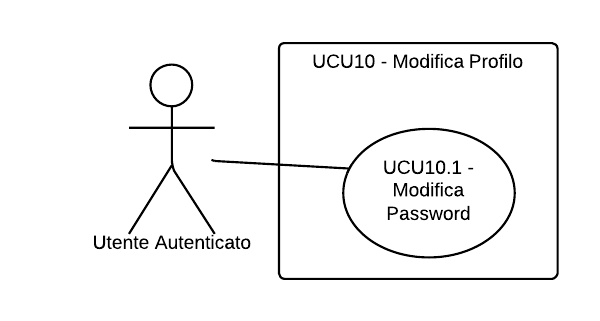
\includegraphics[scale=0.16]{UML/UCU10 - Modifica profilo.png}
      \caption{UCU10 - Modifica profilo}
      \end{center} 
    \end{figure}    
    
      %Tabella 
      \begin{center}
      \bgroup
      \def\arraystretch{1.8}     
      \begin{longtable}{  p{3.5cm} | p{8cm} } 
            
      \hline
      \multicolumn{2}{ | c | }{ \cellcolor[gray]{0.9} \textbf{UCU10 - Modifica profilo}} \\ 
      \hline
      
      \textbf{Attori Primari} & Utente autenticato \\ 
          \textbf{Scopo e Descrizione} & L'utente autenticato ha a disposizione una pagina in cui poter modificare il proprio profilo, modificando email e/o password. \\ 
          
          \textbf{Precondizioni}  & L'applicazione visualizza all'utente la pagina di modifica del proprio profilo.\\ 
          
          \textbf{Postcondizioni} & L'applicazione ha modificato correttamente le credenziali dell'utente e le ha salvate nel database delle credenziali. \\ 
          \textbf{Flusso Principale} & 1. L'utente autenticato modifica la propria email (UCU10.1);  \newline
2. L'utente autenticato modifica la propria password (UCU10.2). \\
          
      \end{longtable}
      \egroup
\end{center}

\subsubsection{UCU10.1 - Modifica password} 
      %Tabella 
      \begin{center}
      \bgroup
      \def\arraystretch{1.8}     
      \begin{longtable}{  p{3.5cm} | p{8cm} } 
            
      \hline
      \multicolumn{2}{ | c | }{ \cellcolor[gray]{0.9} \textbf{UCU10.1 - Modifica password}} \\ 
      \hline
      
      \textbf{Attori Primari} & Utente autenticato \\ 
          \textbf{Scopo e Descrizione} & L'utente autenticato inserisce la nuova password in un apposito campo di testo. \\ 
          
          \textbf{Precondizioni}  & L'utente autenticato si trova all'interno della pagina di modifica del proprio profilo.\\ 
          
          \textbf{Postcondizioni} & L'utente ha inserito la nuova password all'interno dell'apposito campo. \\ 
          \textbf{Flusso Principale} & 1. L'utente autenticato modifica la propria password di accesso all'applicazione (UCU10.1). \\
          
      \end{longtable}
      \egroup
\end{center}

\subsubsection{UCU11 - Gestione utenti}    
    \begin{figure}[H]
      \begin{center}
      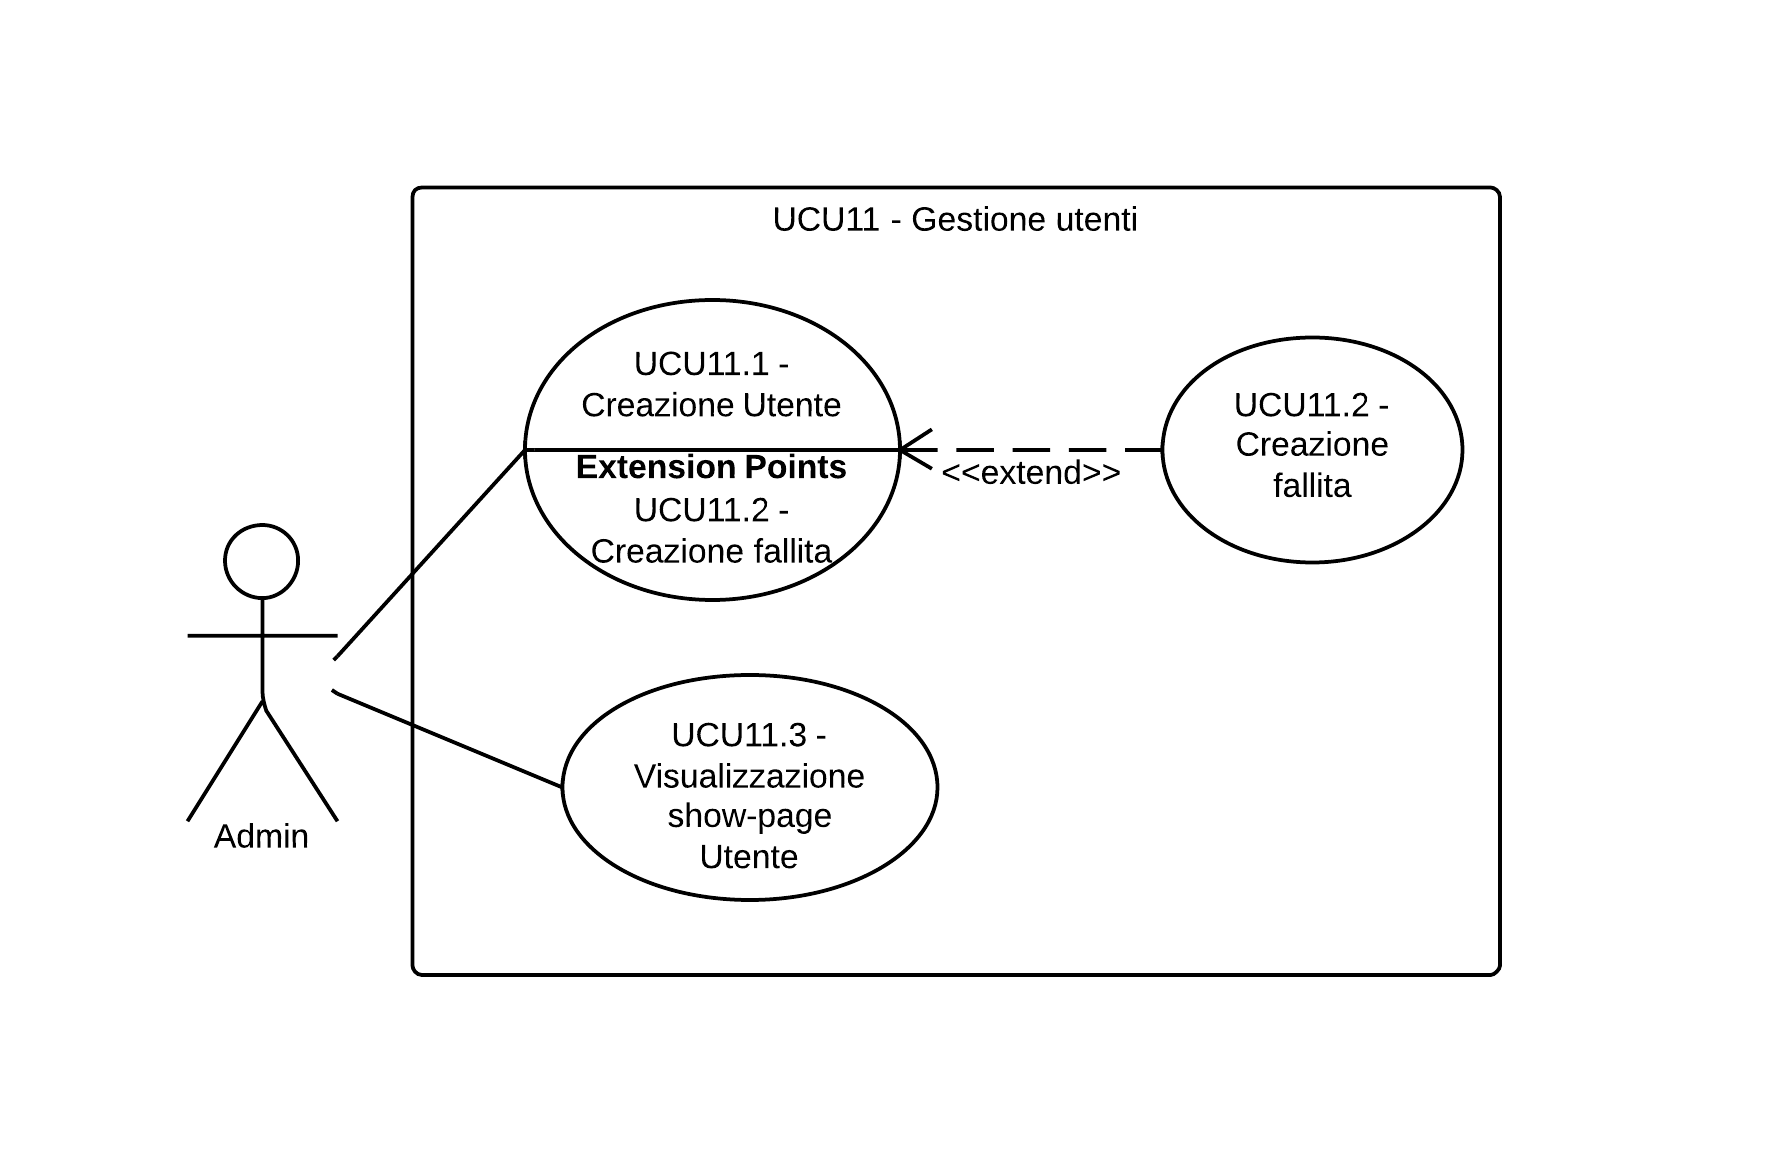
\includegraphics[scale=0.16]{UML/UCU11 - Gestione utenti.png}
      \caption{UCU11 - Gestione utenti}
      \end{center} 
    \end{figure}    
    
      %Tabella 
      \begin{center}
      \bgroup
      \def\arraystretch{1.8}     
      \begin{longtable}{  p{3.5cm} | p{8cm} } 
            
      \hline
      \multicolumn{2}{ | c | }{ \cellcolor[gray]{0.9} \textbf{UCU11 - Gestione utenti}} \\ 
      \hline
      
      \textbf{Attori Primari} & Admin \\ 
          \textbf{Scopo e Descrizione} & L'Admin entra nella sua pagina di amministrazione nella quale visualizza una \glossario{Collection-Index} di tutti gli utenti registrati al sistema. \\ 
          
          \textbf{Precondizioni}  & L'applicazione mostra all'Admin la sua pagina di amministrazione\\ 
          
          \textbf{Postcondizioni} & L'applicazione mette a disposizione dell'Admin tutte le funzionalità di controllo previste. \\ 
          \textbf{Flusso Principale} & 1. L'Admin può creare un nuovo utente (UCU11.1); \newline
2. L'Admin può visualizzare la \glossario{Collection-Show} di un utente (UCU11.3).  \\
           \textbf{Estensioni} & 1.1 - Fallisce l'inserimento di un nuovo utente (UCU11.2). \\
      \end{longtable}
      \egroup
\end{center}

\subsubsection{UCU11.1 - Creazione utente}    
    \begin{figure}[H]
      \begin{center}
      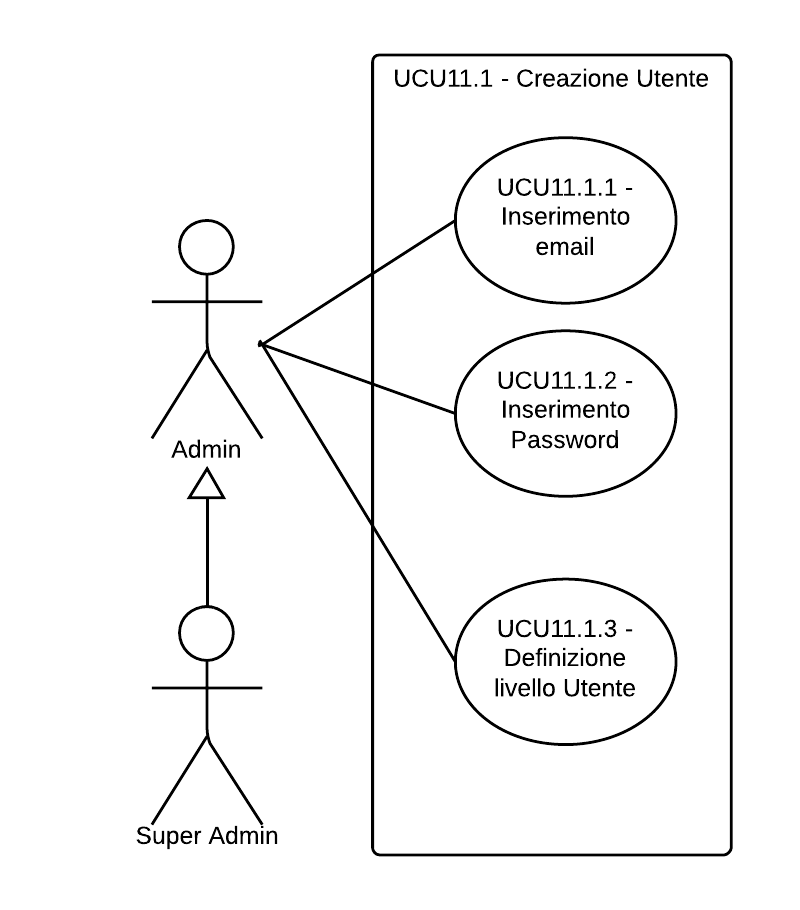
\includegraphics[scale=0.16]{UML/UCU11.1 - Creazione utente.png}
      \caption{UCU11.1 - Creazione utente}
      \end{center} 
    \end{figure}    
    
      %Tabella 
      \begin{center}
      \bgroup
      \def\arraystretch{1.8}     
      \begin{longtable}{  p{3.5cm} | p{8cm} } 
            
      \hline
      \multicolumn{2}{ | c | }{ \cellcolor[gray]{0.9} \textbf{UCU11.1 - Creazione utente}} \\ 
      \hline
      
      \textbf{Attori Primari} & Admin \\ 
          \textbf{Scopo e Descrizione} & L'Admin entra in un'apposita pagina di creazione utente, dalla quale inserisce i dati e crea un nuovo utente nel database delle credenziali. \\ 
          
          \textbf{Precondizioni}  & Il sistema ha reindirizzato l'Admin nella pagina di creazione di un nuovo utente.\\ 
          
          \textbf{Postcondizioni} & Il sistema ha creato un nuovo utente nel database delle credenziali con i dati immessi dall'Admin. \\ 
          \textbf{Flusso Principale} & 1. L'Admin inserisce l'indirizzo email del nuovo utente (UCU11.1.1);  \newline
2. L'Admin inserisce la password del nuovo utente (UCU11.1.2);   \newline
3. L'Admin definisce il livello del nuovo utente (UCU11.1.3).   \\
           \textbf{Scenari Alternativi} & 1. L'Admin lascia la pagina senza aver salvato le modifiche;  \newline
2. I dati inseriti dall'Admin non sono corretti e fallisce la registrazione.  \newline \\
      \end{longtable}
      \egroup
\end{center}

\subsubsection{UCU11.1.1 - Inserimento email} 
      %Tabella 
      \begin{center}
      \bgroup
      \def\arraystretch{1.8}     
      \begin{longtable}{  p{3.5cm} | p{8cm} } 
            
      \hline
      \multicolumn{2}{ | c | }{ \cellcolor[gray]{0.9} \textbf{UCU11.1.1 - Inserimento email}} \\ 
      \hline
      
      \textbf{Attori Primari} & Admin \\ 
          \textbf{Scopo e Descrizione} & L'Admin può inserire in un campo di testo l'indirizzo email dell'utente da creare. \\ 
          
          \textbf{Precondizioni}  & Il sistema mette a disposizione dell'Admin un campo di testo dove inserire la password del nuovo utente.\\ 
          
          \textbf{Postcondizioni} & Il campo di testo è stato compilato correttamente. \\ 
          \textbf{Flusso Principale} & 1. L'admin inserisce l'email per la creazione di un nuovo utente (UCU11.1.1). \\
          
      \end{longtable}
      \egroup
\end{center}

\subsubsection{UCU11.1.2 - Inserimento password} 
      %Tabella 
      \begin{center}
      \bgroup
      \def\arraystretch{1.8}     
      \begin{longtable}{  p{3.5cm} | p{8cm} } 
            
      \hline
      \multicolumn{2}{ | c | }{ \cellcolor[gray]{0.9} \textbf{UCU11.1.2 - Inserimento password}} \\ 
      \hline
      
      \textbf{Attori Primari} & Admin \\ 
          \textbf{Scopo e Descrizione} & L'admin può inserire in un campo di testo la password dell'utente da creare. \\ 
          
          \textbf{Precondizioni}  & L'admin è nella pagina di creazione di un nuovo utente.\\ 
          
          \textbf{Postcondizioni} & L'Admin ha inserito l'indirizzo email dell'utente da creare. \\ 
          \textbf{Flusso Principale} & 1. L'admin inserisce la password di accesso all'applicazione del nuovo utente che sta creando (UCU11.1.2). \\
          
      \end{longtable}
      \egroup
\end{center}

\subsubsection{UCU11.1.3 - Definizione livello utente} 
      %Tabella 
      \begin{center}
      \bgroup
      \def\arraystretch{1.8}     
      \begin{longtable}{  p{3.5cm} | p{8cm} } 
            
      \hline
      \multicolumn{2}{ | c | }{ \cellcolor[gray]{0.9} \textbf{UCU11.1.3 - Definizione livello utente}} \\ 
      \hline
      
      \textbf{Attori Primari} & Admin \\ 
          \textbf{Scopo e Descrizione} & L'Admin può selezionare il livello del nuovo utente, che potrà essere il livello "utente" o "admin". \\ 
          
          \textbf{Precondizioni}  & Il sistema mette a disposizione dell'Admin un campo selezionabile dove poter definire il livello del nuovo utente.\\ 
          
          \textbf{Postcondizioni} & Il campo selezionabile è stato selezionato correttamente. \\ 
          \textbf{Flusso Principale} & 1. L'admin definisce il livello del nuovo utente selezionandolo tra "utente" e "admin" (UCU11.1.3). \\
          
      \end{longtable}
      \egroup
\end{center}

\subsubsection{UCU11.2 - Creazione fallita} 
      %Tabella 
      \begin{center}
      \bgroup
      \def\arraystretch{1.8}     
      \begin{longtable}{  p{3.5cm} | p{8cm} } 
            
      \hline
      \multicolumn{2}{ | c | }{ \cellcolor[gray]{0.9} \textbf{UCU11.2 - Creazione fallita}} \\ 
      \hline
      
      \textbf{Attori Primari} & Admin \\ 
          \textbf{Scopo e Descrizione} & L'Admin ha inserito delle credenziali errate e la creazione di un nuovo utente è fallita.
L'operazione di creazione utente può fallire nei seguenti casi : \newline
-Formato email errato;  \newline
-Email già presente;  \newline
-Formato password errato;  \newline
-Fallimento richiesta di connessione al database delle credenziali utenti. \\ 
          
          \textbf{Precondizioni}  & Il sistema ha rilevato degli errori nell'inserimento di un nuovo utente.\\ 
          
          \textbf{Postcondizioni} & Il sistema visualizza un messaggio d'errore. \\ 
          \textbf{Flusso Principale} & 1. L'admin visualizza un messaggio di errore dato dal fallimento della creazione di un nuovo utente (UCU11.2). \\
          
      \end{longtable}
      \egroup
\end{center}

\subsubsection{UCU11.3 - Apertura show-page Utente}    
    \begin{figure}[H]
      \begin{center}
      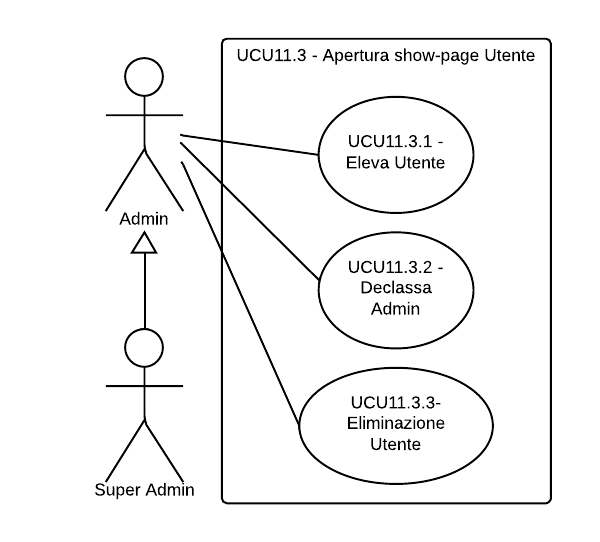
\includegraphics[scale=0.16]{UML/UCU11.3 - Apertura show-page Utente.png}
      \caption{UCU11.3 - Apertura show-page Utente}
      \end{center} 
    \end{figure}    
    
      %Tabella 
      \begin{center}
      \bgroup
      \def\arraystretch{1.8}     
      \begin{longtable}{  p{3.5cm} | p{8cm} } 
            
      \hline
      \multicolumn{2}{ | c | }{ \cellcolor[gray]{0.9} \textbf{UCU11.3 - Apertura show-page Utente}} \\ 
      \hline
      
      \textbf{Attori Primari} & Admin \\ 
          \textbf{Scopo e Descrizione} & L'Admin visualizza la tabella degli utenti registrati e può aprire la relativa show-page di uno di essi tramite link. \\ 
          
          \textbf{Precondizioni}  & L'applicazione mette a disposizione dell'Admin la visualizzazione della show-page dell'utente.\\ 
          
          \textbf{Postcondizioni} & L'applicazione ha reindirizzato l'admin nella \glossario{Collection-Show} dell'utente selezionato. \\ 
          \textbf{Flusso Principale} & 1. L'Admin può elevare un utente normale a livello di Admin (UCU11.3.1);  \newline
2. L'Admin può declassare un Admin a livello di utente normale (UCU11.3.2);  \newline
3. L'Admin può modificare l'email dell'utente selezionato (UCU11.3.3);  \newline
4. L'Admin può modificare la password dell'utente selezionato (UCU11.3.4). \\
          
      \end{longtable}
      \egroup
\end{center}

\subsubsection{UCU11.3.1 - Eleva utente} 
      %Tabella 
      \begin{center}
      \bgroup
      \def\arraystretch{1.8}     
      \begin{longtable}{  p{3.5cm} | p{8cm} } 
            
      \hline
      \multicolumn{2}{ | c | }{ \cellcolor[gray]{0.9} \textbf{UCU11.3.1 - Eleva utente}} \\ 
      \hline
      
      \textbf{Attori Primari} & Admin \\ 
          \textbf{Scopo e Descrizione} & L'Admin eleva l'utente selezionato a livello di Admin. \\ 
          
          \textbf{Precondizioni}  & L'applicazione mette a disposizione dell'Admin la pagina di modifica dell'utente selezionato.\\ 
          
          \textbf{Postcondizioni} & L'applicazione ha elevato l'utente selezionato dall'Admin a livello di "admin". \\ 
          \textbf{Flusso Principale} & 1. L'admin seleziona un utente e lo eleva al livello di "admin" (UCU11.3.1). \\
          
      \end{longtable}
      \egroup
\end{center}

\subsubsection{UCU11.3.2 - Declassa admin} 
      %Tabella 
      \begin{center}
      \bgroup
      \def\arraystretch{1.8}     
      \begin{longtable}{  p{3.5cm} | p{8cm} } 
            
      \hline
      \multicolumn{2}{ | c | }{ \cellcolor[gray]{0.9} \textbf{UCU11.3.2 - Declassa admin}} \\ 
      \hline
      
      \textbf{Attori Primari} & Admin \\ 
          \textbf{Scopo e Descrizione} & L'admin declassa l'admin selezionato al livello di "utente" normale.
L'admin ha potere di declassamento di ruolo su tutti gli admin al di fuori di se stesso e dei Super Admin. \\ 
          
          \textbf{Precondizioni}  & L'applicazione mette a disposizione dell'Admin la possibilità di declassare gli utenti che gli fa visualizzare nella pagina.\\ 
          
          \textbf{Postcondizioni} & L'applicazione ha declassato l'utente selezionato dall'Admin a livello di utente normale. \\ 
          \textbf{Flusso Principale} & 1. L'admin seleziona un altro admin e lo declassa al livello "utente" (UCU11.3.2). \\
          
      \end{longtable}
      \egroup
\end{center}

\subsubsection{UCU11.3.3 - Eliminazione Utente} 
      %Tabella 
      \begin{center}
      \bgroup
      \def\arraystretch{1.8}     
      \begin{longtable}{  p{3.5cm} | p{8cm} } 
            
      \hline
      \multicolumn{2}{ | c | }{ \cellcolor[gray]{0.9} \textbf{UCU11.3.3 - Eliminazione Utente}} \\ 
      \hline
      
      \textbf{Attori Primari} & Admin \\ 
          \textbf{Scopo e Descrizione} & L'Admin decide di eliminare l'utente selezionato. \\ 
          
          \textbf{Precondizioni}  & L'applicazione visualizza la \glossario{Collection-Show} dell'utente selezionato.\\ 
          
          \textbf{Postcondizioni} & L'applicazione ha eliminato l'utente selezionato dall'Admin dal database delle credenziali. \\ 
          \textbf{Flusso Principale} & 1. L'admin elimina l'utente relativo alla show-page visualizzata (UCU11.3.3). \\
          
      \end{longtable}
      \egroup
\end{center}

\subsubsection{UCU12 - Visualizzazione messaggio di errore DSL} 
      %Tabella 
      \begin{center}
      \bgroup
      \def\arraystretch{1.8}     
      \begin{longtable}{  p{3.5cm} | p{8cm} } 
            
      \hline
      \multicolumn{2}{ | c | }{ \cellcolor[gray]{0.9} \textbf{UCU12 - Visualizzazione messaggio di errore DSL}} \\ 
      \hline
      
      \textbf{Attori Primari} & Utente autenticato \\ 
          \textbf{Scopo e Descrizione} & L'utente visualizza un messaggio di errore invece della pagina richiesta, causato da un errore in uno dei file definiti tramite il DSL. \\ 
          
          \textbf{Precondizioni}  & Il sistema ha rilevato un errore in uno o più file definiti tramite linguaggio DSL.\\ 
          
          \textbf{Postcondizioni} & L'applicazione mostra un messaggio di errore all'utente. \\ 
          \textbf{Flusso Principale} & 1. L'utente che ha richiesto la visualizzazione di una pagina visualizza un messaggio di errore causato dal rilevamento di una irregolarità in uno dei file definiti attraverso il DSL (UCU12). \\
          
      \end{longtable}
      \egroup
\end{center}
\subsection{Ambito Sviluppatore}
\subsubsection{UCS - Operazioni ad alto livello} 
    \begin{figure}[H]
      \begin{center}
      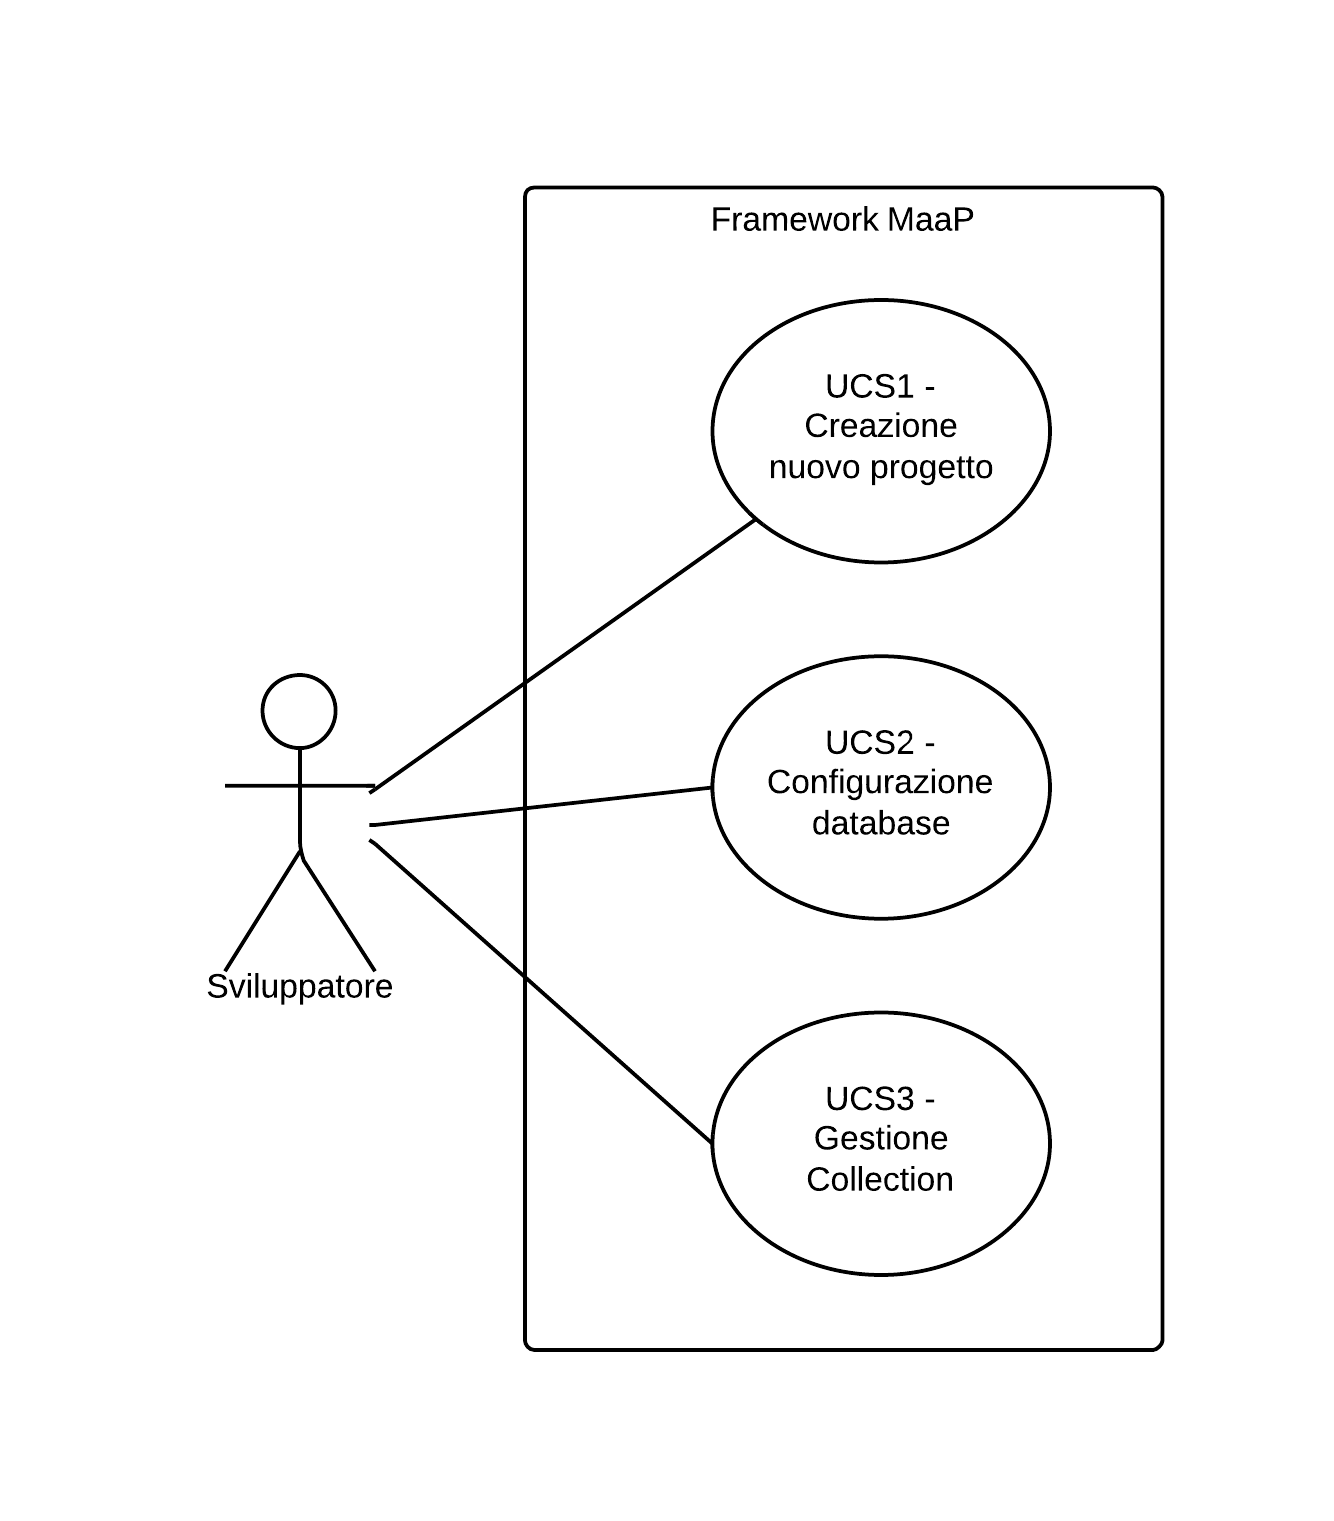
\includegraphics[scale=0.16]{UML/UCS - Operazioni ad alto livello.png}
      \caption{UCS - Operazioni ad alto livello}
      \end{center} 
    \end{figure}  
    
      %Tabella 
      \begin{center}
      \bgroup
      \def\arraystretch{1.8}     
      \begin{longtable}{  p{3.5cm} | p{8cm} } 
            
      \hline
      \multicolumn{2}{ | c | }{ \cellcolor[gray]{0.9} \textbf{UCS - Operazioni ad alto livello}} \\ 
      \hline
      
      \textbf{Attori Primari} & Sviluppatore \\ 
          \textbf{Scopo e Descrizione} & Lo sviluppatore avendo installato lo \glossario{stack tecnologico} richiesto per il funzionamento del \glossario{Framework} \glossario{Maap} può creare un nuovo progetto, dopo averlo creato potrà configurare i database e gestire le \glossario{Collection} che desidera. \\ 
          
          \textbf{Precondizioni}  & Il \glossario{Framework} \glossario{Maap} è funzionante e pronto ad eseguire le azioni dello sviluppatore.\\ 
          
          \textbf{Postcondizioni} & Il \glossario{Framework} ha ottenuto le informazioni sulle azioni che l’utente desidera eseguire. \\
          \textbf{Flusso Principale} & 1. Lo sviluppatore crea un nuovo progetto (UCS1); \newline
2. Lo sviluppatore dopo aver creato il nuovo progetto può configurare i database (UCS2); \newline
3. Lo sviluppatore con il nuovo progetto creato può gestire le \glossario{Collection} che desidera generare (UCS3). \\
          
      \end{longtable}
      \egroup
\end{center}

\subsubsection{UCS1 - Creazione nuovo progetto} 
      %Tabella 
      \begin{center}
      \bgroup
      \def\arraystretch{1.8}     
      \begin{longtable}{  p{3.5cm} | p{8cm} } 
            
      \hline
      \multicolumn{2}{ | c | }{ \cellcolor[gray]{0.9} \textbf{UCS1 - Creazione nuovo progetto}} \\ 
      \hline
      
      \textbf{Attori Primari} & Sviluppatore \\ 
          \textbf{Scopo e Descrizione} & Lo sviluppatore crea un nuovo progetto. \newline
Alla creazione del nuovo progetto ne viene creato lo scheletro che si compone di: \newline
- La creazione delle directory delle pagine web.  \newline
- La creazione del file di configurazione.  \newline
- L'inclusione delle librerie di sistema.  \newline
- La generazione del sistema di autenticazione che include la creazione del database delle credenziali e la generazione dell'utente admin di default. \\ 
          
          \textbf{Precondizioni}  & Il \glossario{Framework} è pronto a creare un nuovo progetto.\\ 
          
          \textbf{Postcondizioni} & Il \glossario{Framework} \glossario{MaaP} ha creato un nuovo progetto completo di tutti i file necessari. \\
      \end{longtable}
      \egroup
\end{center}

\subsubsection{UCS2 - Configurazione database} 
    \begin{figure}[H]
      \begin{center}
      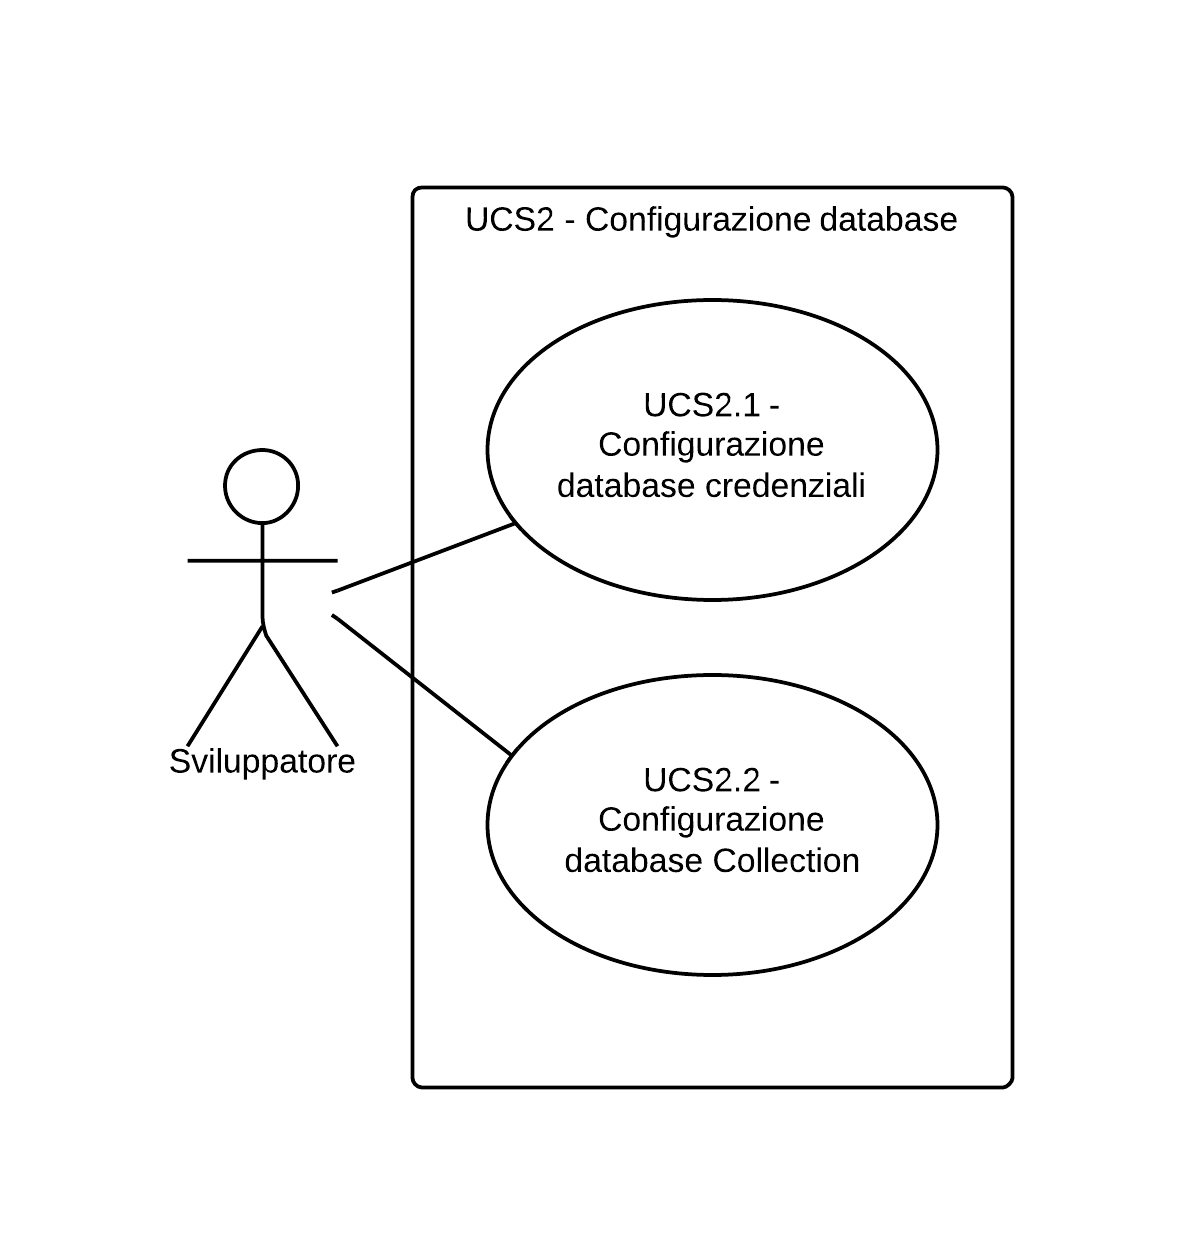
\includegraphics[scale=0.16]{UML/UCS2 - Configurazione database.png}
      \caption{UCS2 - Configurazione database}
      \end{center} 
    \end{figure}  
    
      %Tabella 
      \begin{center}
      \bgroup
      \def\arraystretch{1.8}     
      \begin{longtable}{  p{3.5cm} | p{8cm} } 
            
      \hline
      \multicolumn{2}{ | c | }{ \cellcolor[gray]{0.9} \textbf{UCS2 - Configurazione database}} \\ 
      \hline
      
      \textbf{Attori Primari} & Sviluppatore \\ 
          \textbf{Scopo e Descrizione} & Lo sviluppatore può configurare i due database che compongono il sistema MaaP, ovvero il database delle credenziali utenti e il database contenente le \glossario{Collection}. \\ 
          
          \textbf{Precondizioni}  & Il \glossario{Framework} è funzionante, il progetto è stato creato e lo sviluppatore desidera configurare i database.\\ 
          
          \textbf{Postcondizioni} & Il \glossario{Framework} ha ottenuto le informazioni necessarie ed ha configurato il database delle credenziali e il database delle \glossario{Collection}. \\
          \textbf{Flusso Principale} & 1. Lo sviluppatore può configurare il database delle credenziali utente (UCS2.1); \newline
2. Lo sviluppatore può configurare il database delle \glossario{Collection} (UCS2.2). \\
           \textbf{Esclusioni} & 1.1. Lo sviluppatore può selezionare il namespace per il database delle credenziali utenti (UCS2.3); \newline
2.1. Lo sviluppatore può selezionare il namespace per il database delle \glossario{Collection} (UCS2.3).  \\
      \end{longtable}
      \egroup
\end{center}

\subsubsection{UCS2.1 - Configurazione database credenziali} 
      %Tabella 
      \begin{center}
      \bgroup
      \def\arraystretch{1.8}     
      \begin{longtable}{  p{3.5cm} | p{8cm} } 
            
      \hline
      \multicolumn{2}{ | c | }{ \cellcolor[gray]{0.9} \textbf{UCS2.1 - Configurazione database credenziali}} \\ 
      \hline
      
      \textbf{Attori Primari} & Sviluppatore \\ 
          \textbf{Scopo e Descrizione} & Lo sviluppatore può configurare il database che conterrà le credenziali degli utenti i quali utilizzeranno l'applicazione generata dal \glossario{Framework}.
Se la funzione di \glossario{namespace} è abilitata dovrà essere configurato anche il \glossario{namespace} corrispondente. \\ 
          
          \textbf{Precondizioni}  & Il \glossario{Framework} permette la configurazione del database credenziali.\\ 
          
          \textbf{Postcondizioni} & Il \glossario{Framework} \glossario{Maap} ha configurato il database delle credenziali secondo le informazioni acquisite dallo sviluppatore. \\
      \end{longtable}
      \egroup
\end{center}

\subsubsection{UCS2.2 - Configurazione database Collection} 
      %Tabella 
      \begin{center}
      \bgroup
      \def\arraystretch{1.8}     
      \begin{longtable}{  p{3.5cm} | p{8cm} } 
            
      \hline
      \multicolumn{2}{ | c | }{ \cellcolor[gray]{0.9} \textbf{UCS2.2 - Configurazione database Collection}} \\ 
      \hline
      
      \textbf{Attori Primari} &  \\ 
          \textbf{Scopo e Descrizione} & Lo sviluppatore può configurare il database che conterrà le \glossario{Collection} che l'applicazione generata dal \glossario{Framework} utilizzerà.
Se la funzione di \glossario{namespace} è abilitata dovrà essere configurato anche il \glossario{namespace} corrispondente. \\ 
          
          \textbf{Precondizioni}  & Il \glossario{Framework} è  pronto per l'utilizzo e permette la configurazione del database contenente le \glossario{Collection}.\\ 
          
          \textbf{Postcondizioni} & Il Framework Maap ha configurato il database delle \glossario{Collection} secondo le informazioni acquisite dallo sviluppatore. \\
      \end{longtable}
      \egroup
\end{center}

\subsubsection{UCS2.3 - Selezione namespace} 
      %Tabella 
      \begin{center}
      \bgroup
      \def\arraystretch{1.8}     
      \begin{longtable}{  p{3.5cm} | p{8cm} } 
            
      \hline
      \multicolumn{2}{ | c | }{ \cellcolor[gray]{0.9} \textbf{UCS2.3 - Selezione namespace}} \\ 
      \hline
      
      \textbf{Attori Primari} & Sviluppatore \\ 
          \textbf{Scopo e Descrizione} & Se la funzione di \glossario{namespace} è abilitata lo Sviluppatore può selezionare un \glossario{namespace} per il database da configurare. \\ 
          
          \textbf{Precondizioni}  & Il \glossario{Framework} \glossario{MaaP} mette a disposizione dello sviluppatore un file di configurazione del database.\\ 
          
          \textbf{Postcondizioni} & Il \glossario{Framework} \glossario{MaaP} ha selezionato correttamente il \glossario{namespace} per il database selezionato. \\
      \end{longtable}
      \egroup
\end{center}

\subsubsection{UCS3 - Gestione Collection} 
    \begin{figure}[H]
      \begin{center}
      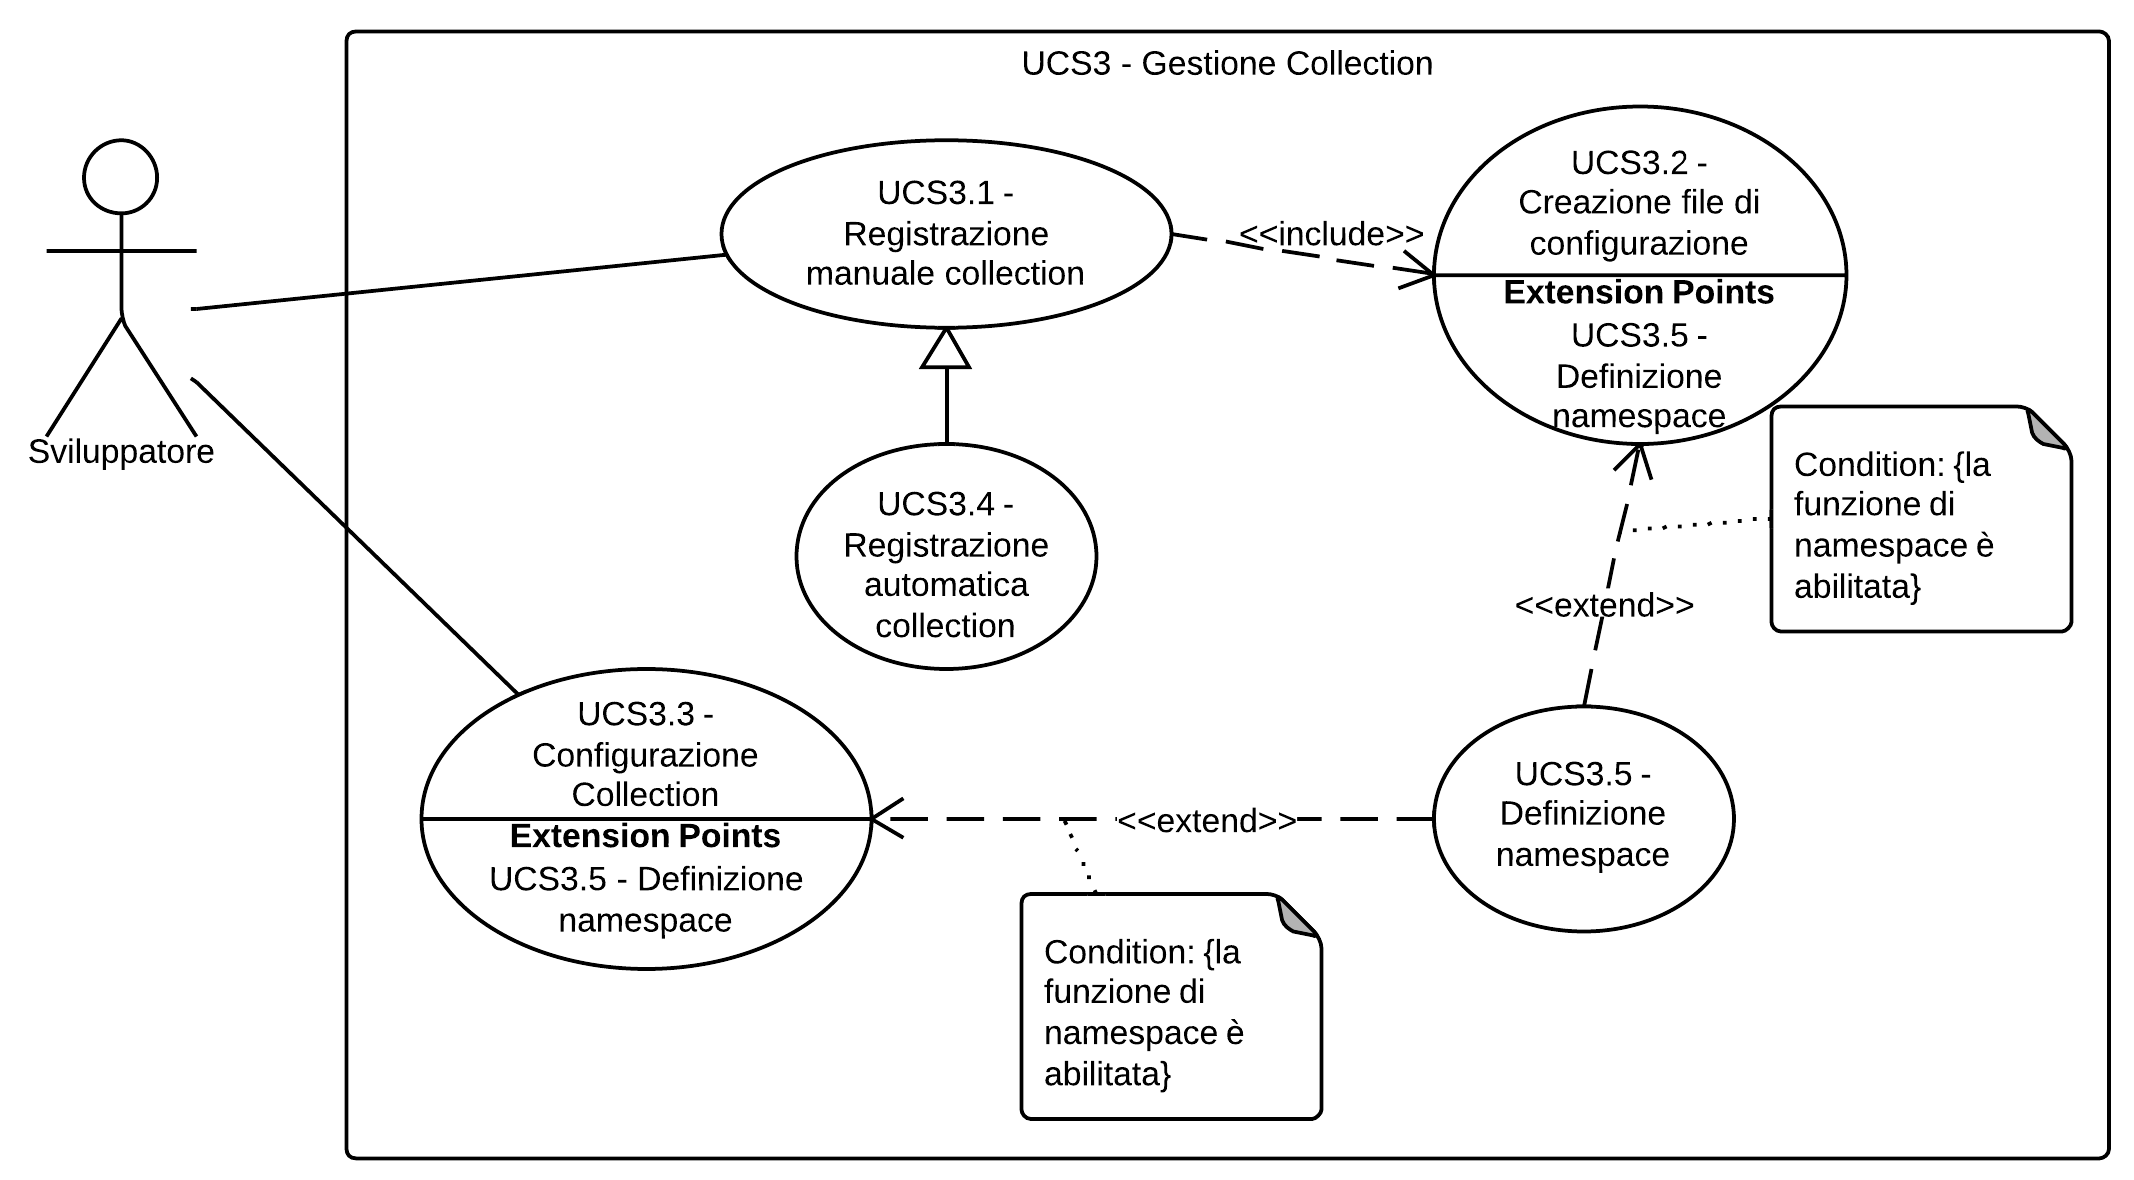
\includegraphics[scale=0.16]{UML/UCS3 - Gestione Collection.png}
      \caption{UCS3 - Gestione Collection}
      \end{center} 
    \end{figure}  
    
      %Tabella 
      \begin{center}
      \bgroup
      \def\arraystretch{1.8}     
      \begin{longtable}{  p{3.5cm} | p{8cm} } 
            
      \hline
      \multicolumn{2}{ | c | }{ \cellcolor[gray]{0.9} \textbf{UCS3 - Gestione Collection}} \\ 
      \hline
      
      \textbf{Attori Primari} & Sviluppatore \\ 
          \textbf{Scopo e Descrizione} & Lo sviluppatore, con il progetto creato, può registrare manualmente una \glossario{Collection} o usufruire della registrazione automatica, con relativa creazione del file di configurazione della stessa. \newline
Può poi configurare le \glossario{Collection} create. \\ 
          
          \textbf{Precondizioni}  & Il \glossario{Framework} \glossario{MaaP} è pronto, il progetto è stato creato e lo sviluppatore intende gestire una \glossario{Collection}.\\ 
          
          \textbf{Postcondizioni} & Il \glossario{Framework} ha appreso le informazioni necessarie sulle azioni che lo sviluppatore vuole eseguire. \\
          \textbf{Flusso Principale} & 1. Lo sviluppatore può registrare manualmente la \glossario{Collection} (UCS3.1); \newline
2. Lo sviluppatore può configurare la \glossario{Collection} registrata (UCS3.3).  \\
           \textbf{Inclusioni} & Viene creato il file di configurazione (UCS3.2). \\ \textbf{Esclusioni} & 1.1. Lo sviluppatore non esegue la registrazione manuale ma eseguire la registrazione automatica della \glossario{Collection} (UCS3.4); \newline
2.1 Lo sviluppatore può definire il namespace della \glossario{Collection} se la funzione di namespace è stata abilitata (UCS3.5). \\
      \end{longtable}
      \egroup
\end{center}

\subsubsection{UCS3.1 - Registrazione manuale Collection} 
      %Tabella 
      \begin{center}
      \bgroup
      \def\arraystretch{1.8}     
      \begin{longtable}{  p{3.5cm} | p{8cm} } 
            
      \hline
      \multicolumn{2}{ | c | }{ \cellcolor[gray]{0.9} \textbf{UCS3.1 - Registrazione manuale Collection}} \\ 
      \hline
      
      \textbf{Attori Primari} & Sviluppatore \\ 
          \textbf{Scopo e Descrizione} & Lo sviluppatore registra manualmente una \glossario{Collection} creando tutti i file necessari al suo funzionamento. \\ 
          
          \textbf{Precondizioni}  & Il \glossario{Framework} \glossario{MaaP} è funzionante e lo sviluppatore ha creato un progetto.\\ 
          
          \textbf{Postcondizioni} & Il \glossario{Framework} \glossario{MaaP} ha registrato correttamente la nuova \glossario{Collection}. \\
      \end{longtable}
      \egroup
\end{center}

\subsubsection{UCS3.2 - Creazione file di configurazione} 
      %Tabella 
      \begin{center}
      \bgroup
      \def\arraystretch{1.8}     
      \begin{longtable}{  p{3.5cm} | p{8cm} } 
            
      \hline
      \multicolumn{2}{ | c | }{ \cellcolor[gray]{0.9} \textbf{UCS3.2 - Creazione file di configurazione}} \\ 
      \hline
      
      \textbf{Attori Primari} & Sviluppatore \\ 
          \textbf{Scopo e Descrizione} & Nella registrazione di una nuova \glossario{Collection} deve essere creato un file di configurazione per essa. \\ 
          
          \textbf{Precondizioni}  & Il \glossario{Framework} \glossario{MaaP} sta registrando una nuova \glossario{Collection}.\\ 
          
          \textbf{Postcondizioni} & Il \glossario{Framework} \glossario{MaaP} ha creato il file di configurazione per la nuova \glossario{Collection}. \\
      \end{longtable}
      \egroup
\end{center}

\subsubsection{UCS3.3 - Configurazione Collection} 
    \begin{figure}[H]
      \begin{center}
      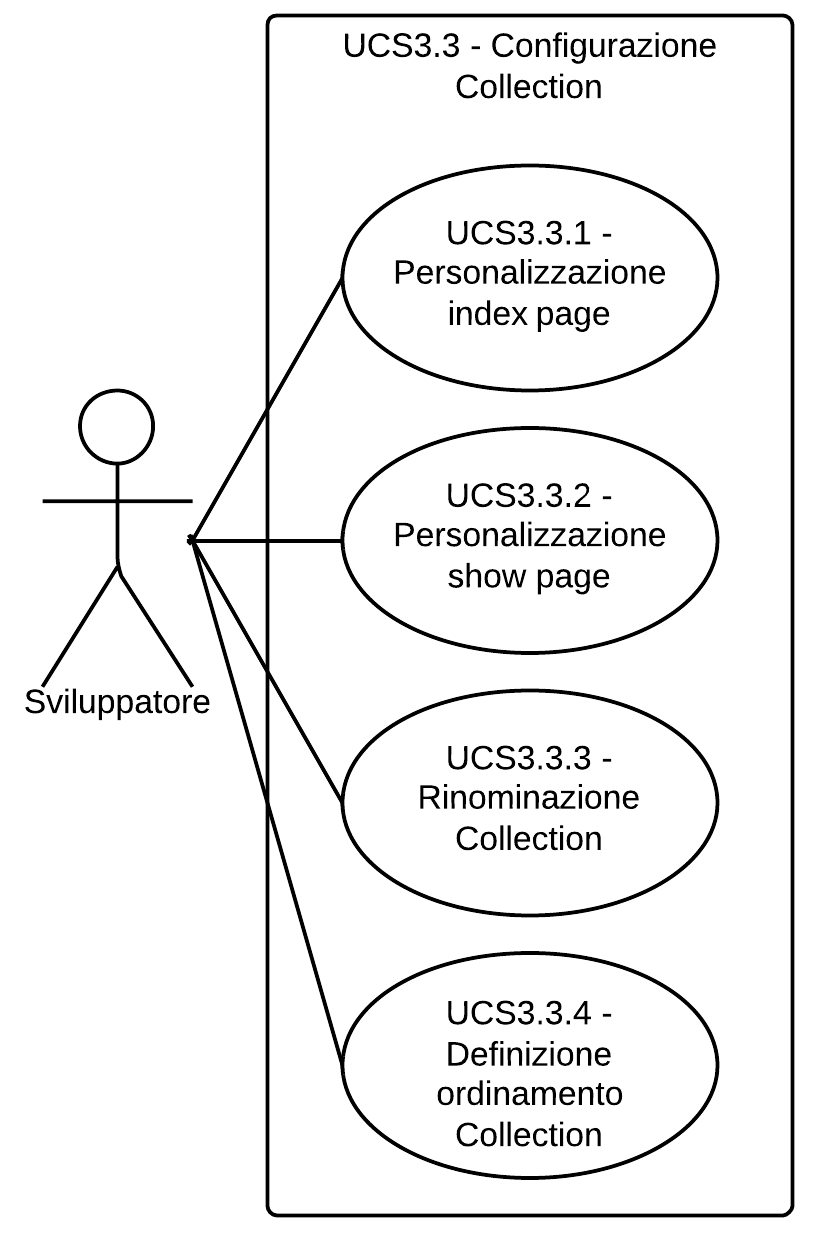
\includegraphics[scale=0.16]{UML/UCS3.3 - Configurazione Collection.png}
      \caption{UCS3.3 - Configurazione Collection}
      \end{center} 
    \end{figure}  
    
      %Tabella 
      \begin{center}
      \bgroup
      \def\arraystretch{1.8}     
      \begin{longtable}{  p{3.5cm} | p{8cm} } 
            
      \hline
      \multicolumn{2}{ | c | }{ \cellcolor[gray]{0.9} \textbf{UCS3.3 - Configurazione Collection}} \\ 
      \hline
      
      \textbf{Attori Primari} & Sviluppatore \\ 
          \textbf{Scopo e Descrizione} & Lo sviluppatore modifica il file di configurazione di una \glossario{Collection} creata. \\ 
          
          \textbf{Precondizioni}  & Il \glossario{Framework} \glossario{MaaP} ha registrato correttamente la \glossario{Collection} da configurare.\\ 
          
          \textbf{Postcondizioni} & Il \glossario{Framework} \glossario{MaaP} ha configurato correttamente la \glossario{Collection} modificata dallo sviluppatore. \\
          \textbf{Flusso Principale} & 1. Lo sviluppatore personalizza la index page della \glossario{Collection} (UCS3.3.1); \newline
2. Lo sviluppatore personalizza la show page della \glossario{Collection} (UCS3.3.2); \newline
3. Lo sviluppatore rinomina il titolo della \glossario{Collection} che verrà visualizzato nel menu di navigazione (UCS3.3.3); \newline
4. Lo sviluppatore definisce l'ordine di visualizzazione della \glossario{Collection} nel menu di navigazione (UCS3.3.4). \\
          
      \end{longtable}
      \egroup
\end{center}

\subsubsection{UCS3.3.1 - Personalizzazione index page} 
    \begin{figure}[H]
      \begin{center}
      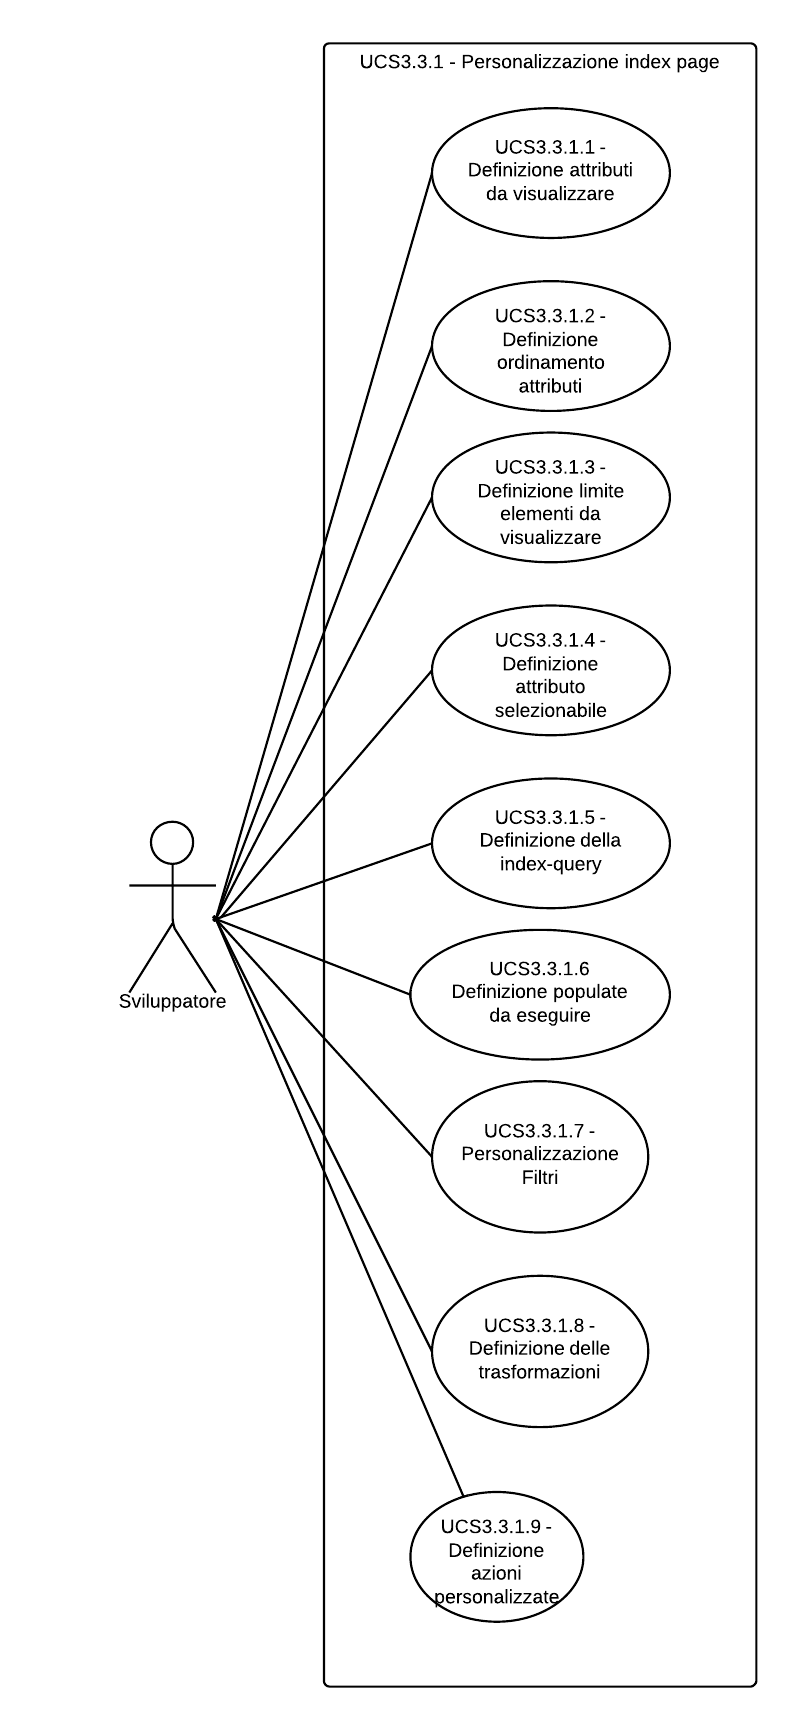
\includegraphics[scale=0.16]{UML/UCS3.3.1 - Personalizzazione index page.png}
      \caption{UCS3.3.1 - Personalizzazione index page}
      \end{center} 
    \end{figure}  
    
      %Tabella 
      \begin{center}
      \bgroup
      \def\arraystretch{1.8}     
      \begin{longtable}{  p{3.5cm} | p{8cm} } 
            
      \hline
      \multicolumn{2}{ | c | }{ \cellcolor[gray]{0.9} \textbf{UCS3.3.1 - Personalizzazione index page}} \\ 
      \hline
      
      \textbf{Attori Primari} & Sviluppatore \\ 
          \textbf{Scopo e Descrizione} & Lo sviluppatore personalizza la index-page della \glossario{Collection} selezionata. \\ 
          
          \textbf{Precondizioni}  & Il \glossario{Framework} \glossario{MaaP} è funzionante e la \glossario{Collection} da configurare è stata registrata.\\ 
          
          \textbf{Postcondizioni} & Il \glossario{Framework} \glossario{MaaP} ha configurato correttamente la index-page della \glossario{Collection}. \\
          \textbf{Flusso Principale} & 1. Lo sviluppatore definisce gli attributi da visualizzare (UCS3.3.1.1); \newline
2. Lo sviluppatore definisce l'ordinamento degli attributi (UCS3.3.1.2); \newline
3. Lo sviluppatore definisce il limite degli elementi da visualizzare (UCS3.3.1.3); \newline
4. Lo sviluppatore definisce quale attributo è selezionabile (UCS3.3.1.4); \newline
5. Lo sviluppatore definisce una query che visualizzerà un sottoinsieme di \glossario{Document} dalla \glossario{Collection} (UCS3.3.1.5); \newline
6. Lo sviluppatore definisce come attributo un attributo innestato o un array di attributi (UCS3.3u.1.6); \newline
7. Lo sviluppatore personalizza la tipologia di filtri da visualizzare (UCS3.3.1.7); \newline
8. Lo sviluppatore definisce delle trasformazioni sugli attributi (UCS3.3.1.8); \newline
9. Lo sviluppatore definisce delle azioni personalizzate (UCS3.3.1.9). \\
          
      \end{longtable}
      \egroup
\end{center}

\subsubsection{UCS3.3.1.1 - Definizione attributi da visualizzare} 
      %Tabella 
      \begin{center}
      \bgroup
      \def\arraystretch{1.8}     
      \begin{longtable}{  p{3.5cm} | p{8cm} } 
            
      \hline
      \multicolumn{2}{ | c | }{ \cellcolor[gray]{0.9} \textbf{UCS3.3.1.1 - Definizione attributi da visualizzare}} \\ 
      \hline
      
      \textbf{Attori Primari} & Sviluppatore \\ 
          \textbf{Scopo e Descrizione} & Lo sviluppatore all'interno del file di configurazione della \glossario{Collection} specifica quali attributi visualizzare nella index-page. \\ 
          
          \textbf{Precondizioni}  & Il \glossario{Framework} \glossario{MaaP} è funzionante e la \glossario{Collection} è registrata.\\ 
          
          \textbf{Postcondizioni} & Il \glossario{Framework} \glossario{MaaP} ha apportato le modifiche alla configurazione della \glossario{Collection}. \\
      \end{longtable}
      \egroup
\end{center}

\subsubsection{UCS3.3.1.2 - Definizione ordinamento attributi} 
      %Tabella 
      \begin{center}
      \bgroup
      \def\arraystretch{1.8}     
      \begin{longtable}{  p{3.5cm} | p{8cm} } 
            
      \hline
      \multicolumn{2}{ | c | }{ \cellcolor[gray]{0.9} \textbf{UCS3.3.1.2 - Definizione ordinamento attributi}} \\ 
      \hline
      
      \textbf{Attori Primari} & Sviluppatore \\ 
          \textbf{Scopo e Descrizione} & Lo sviluppatore all'interno del file di configurazione della \glossario{Collection} definisce un ordinamento di default e specifica quali attributi sono ordinabili o no. \\ 
          
          \textbf{Precondizioni}  & Il \glossario{Framework} \glossario{MaaP} è funzionante e la \glossario{Collection} è registrata.\\ 
          
          \textbf{Postcondizioni} & Il \glossario{Framework} \glossario{MaaP} ha apportato le modifiche alla configurazione della \glossario{Collection}. \\
      \end{longtable}
      \egroup
\end{center}

\subsubsection{UCS3.3.1.3 - Definizione limite elementi da visualizzare} 
      %Tabella 
      \begin{center}
      \bgroup
      \def\arraystretch{1.8}     
      \begin{longtable}{  p{3.5cm} | p{8cm} } 
            
      \hline
      \multicolumn{2}{ | c | }{ \cellcolor[gray]{0.9} \textbf{UCS3.3.1.3 - Definizione limite elementi da visualizzare}} \\ 
      \hline
      
      \textbf{Attori Primari} & Sviluppatore \\ 
          \textbf{Scopo e Descrizione} & Lo sviluppatore all'interno del file di configurazione della \glossario{Collection} specifica quanti \glossario{Document} per pagina verranno visualizzati nella index-page. \\ 
          
          \textbf{Precondizioni}  & Il \glossario{Framework} \glossario{MaaP} è funzionante e la \glossario{Collection} è registrata.\\ 
          
          \textbf{Postcondizioni} & Il \glossario{Framework} \glossario{MaaP} ha apportato le modifiche alla configurazione della \glossario{Collection}. \\
      \end{longtable}
      \egroup
\end{center}

\subsubsection{UCS3.3.1.4 - Definizione attributo selezionabile} 
      %Tabella 
      \begin{center}
      \bgroup
      \def\arraystretch{1.8}     
      \begin{longtable}{  p{3.5cm} | p{8cm} } 
            
      \hline
      \multicolumn{2}{ | c | }{ \cellcolor[gray]{0.9} \textbf{UCS3.3.1.4 - Definizione attributo selezionabile}} \\ 
      \hline
      
      \textbf{Attori Primari} & Sviluppatore \\ 
          \textbf{Scopo e Descrizione} & Lo sviluppatore all'interno del file di configurazione della \glossario{Collection} specifica quale attributo sarà identificato come chiave per poter accedere alla show-page del corrispondente \glossario{Document}. \\ 
          
          \textbf{Precondizioni}  & Il \glossario{Framework} \glossario{MaaP} è funzionante e la \glossario{Collection} è registrata.\\ 
          
          \textbf{Postcondizioni} & Il \glossario{Framework} \glossario{MaaP} ha apportato le modifiche alla configurazione della \glossario{Collection}. \\
      \end{longtable}
      \egroup
\end{center}

\subsubsection{UCS3.3.1.5 - Definizione della index-query} 
      %Tabella 
      \begin{center}
      \bgroup
      \def\arraystretch{1.8}     
      \begin{longtable}{  p{3.5cm} | p{8cm} } 
            
      \hline
      \multicolumn{2}{ | c | }{ \cellcolor[gray]{0.9} \textbf{UCS3.3.1.5 - Definizione della index-query}} \\ 
      \hline
      
      \textbf{Attori Primari} & Sviluppatore \\ 
          \textbf{Scopo e Descrizione} & Lo sviluppatore all'interno del file di configurazione della \glossario{Collection} definisce delle query che andranno a selezionare un sottoinsieme di \glossario{Document} dalla \glossario{Collection}. \\ 
          
          \textbf{Precondizioni}  & Il \glossario{Framework} \glossario{MaaP} è funzionante e la Collection è registrata.\\ 
          
          \textbf{Postcondizioni} & Il \glossario{Framework} \glossario{MaaP} ha apportato le modifiche alla configurazione della \glossario{Collection}. \\
      \end{longtable}
      \egroup
\end{center}

\subsubsection{UCS3.3.1.6 - Definizione populate da eseguire} 
      %Tabella 
      \begin{center}
      \bgroup
      \def\arraystretch{1.8}     
      \begin{longtable}{  p{3.5cm} | p{8cm} } 
            
      \hline
      \multicolumn{2}{ | c | }{ \cellcolor[gray]{0.9} \textbf{UCS3.3.1.6 - Definizione populate da eseguire}} \\ 
      \hline
      
      \textbf{Attori Primari} & Sviluppatore \\ 
          \textbf{Scopo e Descrizione} & Lo sviluppatore all'interno del file di configurazione della \glossario{Collection} specifica attributi che contengono attributi innestati o un array di \glossario{Document} tramite la funzione \glossario{populate}. \\ 
          
          \textbf{Precondizioni}  & Il \glossario{Framework} \glossario{MaaP} è funzionante e la \glossario{Collection} è registrata.\\ 
          
          \textbf{Postcondizioni} & Il \glossario{Framework} \glossario{MaaP} ha apportato le modifiche alla configurazione della \glossario{Collection}. \\
      \end{longtable}
      \egroup
\end{center}

\subsubsection{UCS3.3.1.7 - Personalizzazione filtri} 
      %Tabella 
      \begin{center}
      \bgroup
      \def\arraystretch{1.8}     
      \begin{longtable}{  p{3.5cm} | p{8cm} } 
            
      \hline
      \multicolumn{2}{ | c | }{ \cellcolor[gray]{0.9} \textbf{UCS3.3.1.7 - Personalizzazione filtri}} \\ 
      \hline
      
      \textbf{Attori Primari} & Sviluppatore \\ 
          \textbf{Scopo e Descrizione} & Lo sviluppatore all'interno del file di configurazione della \glossario{Collection} specifica quali filtri inserire nella index-page. \\ 
          
          \textbf{Precondizioni}  & Il \glossario{Framework} \glossario{MaaP} è funzionante e la \glossario{Collection} è registrata.\\ 
          
          \textbf{Postcondizioni} & Il \glossario{Framework} \glossario{MaaP} ha apportato le modifiche alla configurazione della \glossario{Collection}. \\
      \end{longtable}
      \egroup
\end{center}

\subsubsection{UCS3.3.1.8 - Definizione delle trasformazioni} 
      %Tabella 
      \begin{center}
      \bgroup
      \def\arraystretch{1.8}     
      \begin{longtable}{  p{3.5cm} | p{8cm} } 
            
      \hline
      \multicolumn{2}{ | c | }{ \cellcolor[gray]{0.9} \textbf{UCS3.3.1.8 - Definizione delle trasformazioni}} \\ 
      \hline
      
      \textbf{Attori Primari} & Sviluppatore \\ 
          \textbf{Scopo e Descrizione} & Lo sviluppatore all'interno del file di configurazione della \glossario{Collection} specifica delle trasformazioni sui valori degli attributi che visualizzeranno l'attributo in base all'output della funzione di trasformazione. \\ 
          
          \textbf{Precondizioni}  & Il \glossario{Framework} \glossario{MaaP} è funzionante e la \glossario{Collection} è registrata.\\ 
          
          \textbf{Postcondizioni} & Il \glossario{Framework} \glossario{MaaP} ha apportato le modifiche alla configurazione della \glossario{Collection}. \\
      \end{longtable}
      \egroup
\end{center}

\subsubsection{UCS3.3.1.9 - Definizione azioni personalizzate} 
      %Tabella 
      \begin{center}
      \bgroup
      \def\arraystretch{1.8}     
      \begin{longtable}{  p{3.5cm} | p{8cm} } 
            
      \hline
      \multicolumn{2}{ | c | }{ \cellcolor[gray]{0.9} \textbf{UCS3.3.1.9 - Definizione azioni personalizzate}} \\ 
      \hline
      
      \textbf{Attori Primari} & Sviluppatore \\ 
          \textbf{Scopo e Descrizione} & Lo sviluppatore all'interno del file di configurazione della \glossario{Collection} definisce delle azioni personalizzate che potranno essere eseguite dall'applicazione. Deve essere possibile specificare dei permessi per l'esecuzione di ciascuna azione personalizzata, in caso venga omessa chiunque potrà eseguirla. \\ 
          
          \textbf{Precondizioni}  & Il \glossario{Framework} \glossario{MaaP} è funzionante e la \glossario{Collection} è registrata.\\ 
          
          \textbf{Postcondizioni} & Il \glossario{Framework} \glossario{MaaP} ha apportato le modifiche alla configurazione della \glossario{Collection}. \\
      \end{longtable}
      \egroup
\end{center}

\subsubsection{UCS3.3.2 - Personalizzazione show page} 
    \begin{figure}[H]
      \begin{center}
      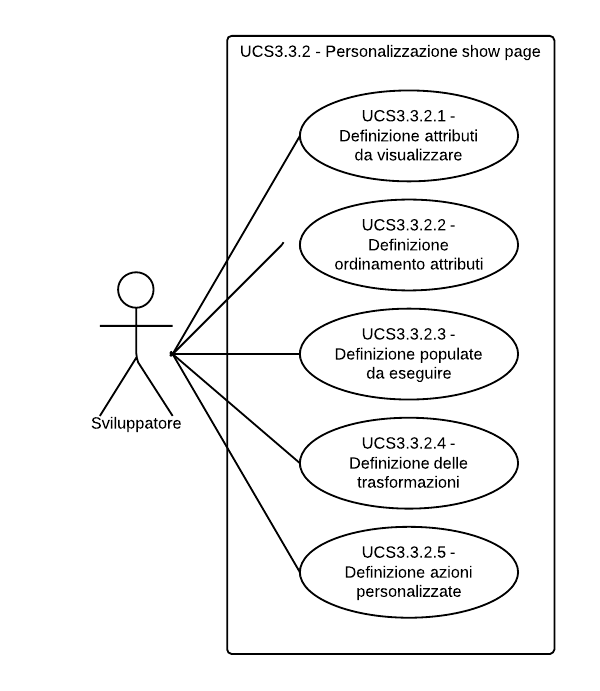
\includegraphics[scale=0.16]{UML/UCS3.3.2 - Personalizzazione show page.png}
      \caption{UCS3.3.2 - Personalizzazione show page}
      \end{center} 
    \end{figure}  
    
      %Tabella 
      \begin{center}
      \bgroup
      \def\arraystretch{1.8}     
      \begin{longtable}{  p{3.5cm} | p{8cm} } 
            
      \hline
      \multicolumn{2}{ | c | }{ \cellcolor[gray]{0.9} \textbf{UCS3.3.2 - Personalizzazione show page}} \\ 
      \hline
      
      \textbf{Attori Primari} & Sviluppatore \\ 
          \textbf{Scopo e Descrizione} & Lo sviluppatore personalizza la show-page della \glossario{Collection} selezionata. \\ 
          
          \textbf{Precondizioni}  & Il \glossario{Framework} \glossario{MaaP} è funzionante e la \glossario{Collection} da configurare è stata registrata.\\ 
          
          \textbf{Postcondizioni} & Il \glossario{Framework} \glossario{MaaP} ha configurato correttamente la show-page della \glossario{Collection}. \\
          \textbf{Flusso Principale} & 1. Lo sviluppatore definisce gli attributi da visualizzare nella show-page (UCS3.3.2.1); \newline
2. Lo sviluppatore definisce l'ordinamento degli attributi nella show-page (UCS3.3.2.2); \newline
3. Lo sviluppatore definisce attributi che contengono attributi innestati o array di attributi (UCS3.3.2.3); \newline
4. Lo sviluppatore definisce delle trasformazioni sugli attributi (UCS3.3.2.4); \newline
5. Lo sviluppatore definisce delle azioni personalizzate da eseguire all'interno della show-page (UCS3.3.2.5). \newline \\
          
      \end{longtable}
      \egroup
\end{center}

\subsubsection{UCS3.3.2.1 - Definizione attributi da visualizzare} 
      %Tabella 
      \begin{center}
      \bgroup
      \def\arraystretch{1.8}     
      \begin{longtable}{  p{3.5cm} | p{8cm} } 
            
      \hline
      \multicolumn{2}{ | c | }{ \cellcolor[gray]{0.9} \textbf{UCS3.3.2.1 - Definizione attributi da visualizzare}} \\ 
      \hline
      
      \textbf{Attori Primari} & Sviluppatore \\ 
          \textbf{Scopo e Descrizione} & Lo sviluppatore all'interno del file di configurazione della \glossario{Collection} specifica quali attributi visualizzare nella show-page. \\ 
          
          \textbf{Precondizioni}  & Il \glossario{Framework} \glossario{MaaP} è funzionante e la \glossario{Collection} è registrata.\\ 
          
          \textbf{Postcondizioni} & Il \glossario{Framework} \glossario{MaaP} ha apportato le modifiche alla configurazione della \glossario{Collection}. \\
      \end{longtable}
      \egroup
\end{center}

\subsubsection{UCS3.3.2.2 - Definizione ordinamento attributi} 
      %Tabella 
      \begin{center}
      \bgroup
      \def\arraystretch{1.8}     
      \begin{longtable}{  p{3.5cm} | p{8cm} } 
            
      \hline
      \multicolumn{2}{ | c | }{ \cellcolor[gray]{0.9} \textbf{UCS3.3.2.2 - Definizione ordinamento attributi}} \\ 
      \hline
      
      \textbf{Attori Primari} & Sviluppatore \\ 
          \textbf{Scopo e Descrizione} & Lo sviluppatore all'interno del file di configurazione della \glossario{Collection} specifica l'ordinamento degli attributi da visualizzare nella show-page. \\ 
          
          \textbf{Precondizioni}  & Il \glossario{Framework} \glossario{MaaP} è funzionante e la \glossario{Collection} è registrata.\\ 
          
          \textbf{Postcondizioni} & Il \glossario{Framework} \glossario{MaaP} ha apportato le modifiche alla configurazione della \glossario{Collection}. \\
      \end{longtable}
      \egroup
\end{center}

\subsubsection{UCS3.3.2.3 - Definizione populate da eseguire} 
      %Tabella 
      \begin{center}
      \bgroup
      \def\arraystretch{1.8}     
      \begin{longtable}{  p{3.5cm} | p{8cm} } 
            
      \hline
      \multicolumn{2}{ | c | }{ \cellcolor[gray]{0.9} \textbf{UCS3.3.2.3 - Definizione populate da eseguire}} \\ 
      \hline
      
      \textbf{Attori Primari} & Sviluppatore \\ 
          \textbf{Scopo e Descrizione} & Lo sviluppatore all'interno del file di configurazione della \glossario{Collection} specifica attributi che contengono attributi innestati o un array di \glossario{Document} tramite la funzione \glossario{populate}. \\ 
          
          \textbf{Precondizioni}  & Il \glossario{Framework} \glossario{MaaP} è funzionante e la \glossario{Collection} è registrata.\\ 
          
          \textbf{Postcondizioni} & Il \glossario{Framework} \glossario{MaaP} ha apportato le modifiche alla configurazione della \glossario{Collection}. \\
      \end{longtable}
      \egroup
\end{center}

\subsubsection{UCS3.3.2.4 - Definizione delle trasformazioni} 
      %Tabella 
      \begin{center}
      \bgroup
      \def\arraystretch{1.8}     
      \begin{longtable}{  p{3.5cm} | p{8cm} } 
            
      \hline
      \multicolumn{2}{ | c | }{ \cellcolor[gray]{0.9} \textbf{UCS3.3.2.4 - Definizione delle trasformazioni}} \\ 
      \hline
      
      \textbf{Attori Primari} & Sviluppatore \\ 
          \textbf{Scopo e Descrizione} & Lo sviluppatore all'interno del file di configurazione della \glossario{Collection} specifica delle trasformazioni sui valori degli attributi che visualizzeranno l'attributo in base all'output della funzione di trasformazione. \\ 
          
          \textbf{Precondizioni}  & Il \glossario{Framework} \glossario{MaaP} è funzionante e la \glossario{Collection} è registrata.\\ 
          
          \textbf{Postcondizioni} & Il \glossario{Framework} \glossario{MaaP} ha apportato le modifiche alla configurazione della \glossario{Collection}. \\
      \end{longtable}
      \egroup
\end{center}

\subsubsection{UCS3.3.2.5 - Definizione azioni personalizzate} 
      %Tabella 
      \begin{center}
      \bgroup
      \def\arraystretch{1.8}     
      \begin{longtable}{  p{3.5cm} | p{8cm} } 
            
      \hline
      \multicolumn{2}{ | c | }{ \cellcolor[gray]{0.9} \textbf{UCS3.3.2.5 - Definizione azioni personalizzate}} \\ 
      \hline
      
      \textbf{Attori Primari} & Sviluppatore \\ 
          \textbf{Scopo e Descrizione} & Lo sviluppatore all'interno del file di configurazione della \glossario{Collection} definisce delle azioni personalizzate che potranno essere eseguite dalla show-page. Deve essere possibile specificare dei permessi per l'esecuzione di ciascuna azione personalizzata, in caso venga omessa chiunque potrà eseguirla. \\ 
          
          \textbf{Precondizioni}  & Il \glossario{Framework} \glossario{MaaP} è funzionante e la \glossario{Collection} è registrata.\\ 
          
          \textbf{Postcondizioni} & Il \glossario{Framework} \glossario{MaaP} ha apportato le modifiche alla configurazione della \glossario{Collection}. \\
      \end{longtable}
      \egroup
\end{center}

\subsubsection{UCS3.3.3 - Rinominazione Collection} 
      %Tabella 
      \begin{center}
      \bgroup
      \def\arraystretch{1.8}     
      \begin{longtable}{  p{3.5cm} | p{8cm} } 
            
      \hline
      \multicolumn{2}{ | c | }{ \cellcolor[gray]{0.9} \textbf{UCS3.3.3 - Rinominazione Collection}} \\ 
      \hline
      
      \textbf{Attori Primari} & Sviluppatore \\ 
          \textbf{Scopo e Descrizione} & Lo sviluppatore può rinominare una \glossario{Collection} creata. \\ 
          
          \textbf{Precondizioni}  & Il \glossario{Framework} è funzionante, la \glossario{Collection} da ridenominare è stata registrata e lo sviluppatore intende rinominarla.\\ 
          
          \textbf{Postcondizioni} & Il \glossario{Framework} attraverso le informazioni date dallo sviluppatore ha rinominato la \glossario{Collection} desiderata. \\
      \end{longtable}
      \egroup
\end{center}

\subsubsection{UCS3.3.4 - Definizione ordinamento Collection} 
      %Tabella 
      \begin{center}
      \bgroup
      \def\arraystretch{1.8}     
      \begin{longtable}{  p{3.5cm} | p{8cm} } 
            
      \hline
      \multicolumn{2}{ | c | }{ \cellcolor[gray]{0.9} \textbf{UCS3.3.4 - Definizione ordinamento Collection}} \\ 
      \hline
      
      \textbf{Attori Primari} & Sviluppatore \\ 
          \textbf{Scopo e Descrizione} & Lo sviluppatore può definire l'ordinamento della \glossario{Collection} rispetto alle altre \glossario{Collection} già registrate. \\ 
          
          \textbf{Precondizioni}  & Il \glossario{Framework} è funzionante e la \glossario{Collection} di cui definire l'ordinamento è stata registrata.\\ 
          
          \textbf{Postcondizioni} & Il \glossario{Framework} ha appreso le informazioni date dallo sviluppatore e ha definito l'ordinamento della \glossario{Collection}. \\
          \textbf{Flusso Principale} & 1. Lo sviluppatore definisce l'ordinamento della \glossario{Collection} rispetto alle altre \glossario{Collection} già registrate (UCS3.3.4) \\
          
      \end{longtable}
      \egroup
\end{center}

\subsubsection{UCS3.3.5 - Definizione namespace} 
      %Tabella 
      \begin{center}
      \bgroup
      \def\arraystretch{1.8}     
      \begin{longtable}{  p{3.5cm} | p{8cm} } 
            
      \hline
      \multicolumn{2}{ | c | }{ \cellcolor[gray]{0.9} \textbf{UCS3.3.5 - Definizione namespace}} \\ 
      \hline
      
      \textbf{Attori Primari} & Sviluppatore \\ 
          \textbf{Scopo e Descrizione} & Lo sviluppatore, se la funzione di \glossario{namespace} è abilitata, può definire un \glossario{namespace} per l'applicazione \glossario{MaaP} generata ed associarlo alle \glossario{Collection} da creare. \\ 
          
          \textbf{Precondizioni}  & Il \glossario{Framework} \glossario{MaaP} ha generato un'applicazione funzionante.\\ 
          
          \textbf{Postcondizioni} & La \glossario{collection} ha un \glossario{namespace} definito al suo interno. \\
          \textbf{Flusso Principale} & 1. Lo Sviluppatore associa il \glossario{namespace} da lui definito alle \glossario{Collection} da creare (UCS3.3.5) \\
          
      \end{longtable}
      \egroup
\end{center}

\subsubsection{UCS3.4 - Registrazione automatica Collection} 
      %Tabella 
      \begin{center}
      \bgroup
      \def\arraystretch{1.8}     
      \begin{longtable}{  p{3.5cm} | p{8cm} } 
            
      \hline
      \multicolumn{2}{ | c | }{ \cellcolor[gray]{0.9} \textbf{UCS3.4 - Registrazione automatica Collection}} \\ 
      \hline
      
      \textbf{Attori Primari} & Sviluppatore \\ 
          \textbf{Scopo e Descrizione} & Lo sviluppatore crea automaticamente una nuova \glossario{Collection} da linea di comando. \\ 
          
          \textbf{Precondizioni}  & Il \glossario{Framework} \glossario{MaaP} è funzionante e lo sviluppatore ha creato un progetto.\\ 
          
          \textbf{Postcondizioni} & Il \glossario{Framework} \glossario{MaaP} ha registrato correttamente la nuova \glossario{Collection}. \\
          \textbf{Flusso Principale} & 1. Lo sviluppatore crea automaticamente una nuova \glossario{Collection} da linea di comando (UCS3.4) \\
          
      \end{longtable}
      \egroup
\end{center}

\subsubsection{UCS3.6 - Visualizzazione messaggio di errore DSL} 
      %Tabella 
      \begin{center}
      \bgroup
      \def\arraystretch{1.8}     
      \begin{longtable}{  p{3.5cm} | p{8cm} } 
            
      \hline
      \multicolumn{2}{ | c | }{ \cellcolor[gray]{0.9} \textbf{UCS3.6 - Visualizzazione messaggio di errore DSL}} \\ 
      \hline
      
      \textbf{Attori Primari} & Sviluppatore \\ 
          \textbf{Scopo e Descrizione} & Lo sviluppatore quando configura una Collection potrebbe incappare in errori di sintassi o di tipo logico legati al linguaggio DSL con cui sta programmando. In tal caso \glossario{MaaP} deve segnalare allo sviluppatore un messaggio d'errore. \\ 
          
          \textbf{Precondizioni}  & Il \glossario{Framework} \glossario{MaaP} verifica il codice prodotto dallo sviluppatore.\\ 
          
          \textbf{Postcondizioni} & Il \glossario{Framework} \glossario{MaaP} ha riscontrato un errore logico o di sintassi all'interno del codice prodotto dallo sviluppatore e lancia un messaggio di errore. \\
          \textbf{Flusso Principale} & 1. Lo Sviluppatore visualizza il messaggio d'errore relativo al DSL fornito. \\
          
      \end{longtable}
      \egroup
\end{center}

\subsubsection{UCS4 - Abilitazione namespace} 
      %Tabella 
      \begin{center}
      \bgroup
      \def\arraystretch{1.8}     
      \begin{longtable}{  p{3.5cm} | p{8cm} } 
            
      \hline
      \multicolumn{2}{ | c | }{ \cellcolor[gray]{0.9} \textbf{UCS4 - Abilitazione namespace}} \\ 
      \hline
      
      \textbf{Attori Primari} & Sviluppatore \\ 
          \textbf{Scopo e Descrizione} & L'attore sviluppatore può scegliere se far utilizzare i \glossario{namespace} all'applicazione \glossario{MaaP}. Il \glossario{namespace} viene utilizzato da \glossario{MaaP} per sapere quali file considerare quando gli viene richiesta una pagina. \\ 
          
          \textbf{Precondizioni}  & L'applicazione \glossario{MaaP} è stata creata ed è funzionante.\\ 
          
          \textbf{Postcondizioni} & L'applicazione \glossario{MaaP} dispone delle funzionalità di \glossario{namespace}. \\
          \textbf{Flusso Principale} & 1. Lo sviluppatore attiva il \glossario{namespace} (UCS4) \\
          
      \end{longtable}
      \egroup
\end{center}
\subsection{Ambito Utente MaaS}
\subsubsection{UCM - Operazioni ad alto livello - Utente MaaS non autenticato} 
    \begin{figure}[H]
      \begin{center}
      \includegraphics[scale=0.16]{UML/UCM - Operazioni ad alto livello - Utente MaaS non autenticato.png}
      \caption{UCM - Operazioni ad alto livello - Utente MaaS non autenticato}
      \end{center} 
    \end{figure}  
    
      %Tabella 
      \begin{center}
      \bgroup
      \def\arraystretch{1.8}     
      \begin{longtable}{  p{3.5cm} | p{8cm} } 
            
      \hline
      \multicolumn{2}{ | c | }{ \cellcolor[gray]{0.9} \textbf{UCM - Operazioni ad alto livello - Utente MaaS non autenticato}} \\ 
      \hline
      
      \textbf{Attori Primari} & Utente MaaS non autenticato \\ 
          \textbf{Scopo e Descrizione} & L'utente \glossario{MaaS} non autenticato può registrarsi al servizio \glossario{MaaS} o effettuare il login. \\ 
          
          \textbf{Precondizioni}  & \glossario{MaaS} è funzionante ed attende che l'utente non autenticato interagisca.\\ 
          
          \textbf{Postcondizioni} & Il servizio \glossario{MaaS} ha acquisito le informazioni necessarie per svolgere le azioni che l'utente \glossario{MaaS} non autenticato ha richiesto. \\
          \textbf{Flusso Principale} & 1. L'utente \glossario{MaaS} non autenticato può registrarsi al servizio (UCM1); \newline
2. L'utente \glossario{MaaS} non autenticato può effettuare il login (UCM4). \\
           \textbf{Esclusioni} & 1.1 L'utente non autenticato visualizza un messaggio di errore dovuto all'esistenza delle credenziali inserite per registrarsi al servizio (UCM3); \newline
2.1 L'utente visualizza un messaggio di errore dopo aver inserito dati non corretti nell'operazione di login (UCM5). \\
      \end{longtable}
      \egroup
\end{center}

\subsubsection{UCM - Operazioni ad alto livello - Utente MaaS autenticato} 
    \begin{figure}[H]
      \begin{center}
      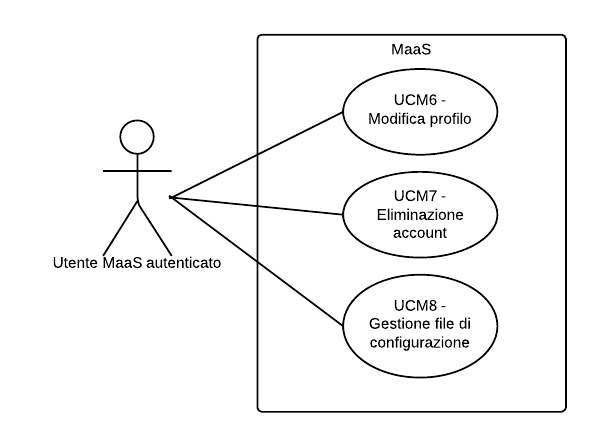
\includegraphics[scale=0.16]{UML/UCM - Operazioni ad alto livello - Utente MaaS autenticato.png}
      \caption{UCM - Operazioni ad alto livello - Utente MaaS autenticato}
      \end{center} 
    \end{figure}  
    
      %Tabella 
      \begin{center}
      \bgroup
      \def\arraystretch{1.8}     
      \begin{longtable}{  p{3.5cm} | p{8cm} } 
            
      \hline
      \multicolumn{2}{ | c | }{ \cellcolor[gray]{0.9} \textbf{UCM - Operazioni ad alto livello - Utente MaaS autenticato}} \\ 
      \hline
      
      \textbf{Attori Primari} & Utente MaaS autenticato \\ 
          \textbf{Scopo e Descrizione} & L'utente \glossario{MaaS} autenticato può modificare il suo profilo, eliminare il proprio account o gestire i file di configurazione per la creazione della pagine. \\ 
          
          \textbf{Precondizioni}  & \glossario{MaaS} è funzionante ed attende che l'utente interagisca.\\ 
          
          \textbf{Postcondizioni} & Il servizio \glossario{MaaS} ha acquisito le informazioni necessarie per svolgere le azioni che l'utente \glossario{MaaS} autenticato ha richiesto. \\
          \textbf{Flusso Principale} & 1. L'utente \glossario{MaaS} autenticato può modificare il proprio profilo (UCM6); \newline
2. L'utente \glossario{MaaS} autenticato può eliminare il proprio account (UCM7); \newline
3. L'utente \glossario{MaaS} autenticato può gestire i file di configurazione (UCM8).  \\
          
      \end{longtable}
      \egroup
\end{center}

\subsubsection{UCM1 - Registrazione} 
    \begin{figure}[H]
      \begin{center}
      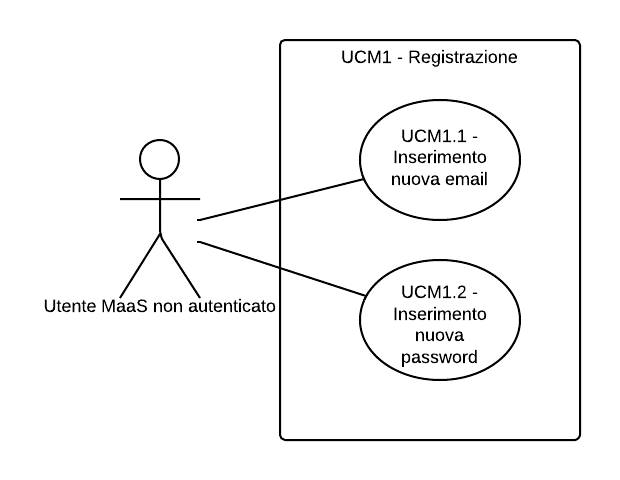
\includegraphics[scale=0.16]{UML/UCM1 - Registrazione.png}
      \caption{UCM1 - Registrazione}
      \end{center} 
    \end{figure}  
    
      %Tabella 
      \begin{center}
      \bgroup
      \def\arraystretch{1.8}     
      \begin{longtable}{  p{3.5cm} | p{8cm} } 
            
      \hline
      \multicolumn{2}{ | c | }{ \cellcolor[gray]{0.9} \textbf{UCM1 - Registrazione}} \\ 
      \hline
      
      \textbf{Attori Primari} & Utente MaaS non autenticato \\ 
          \textbf{Scopo e Descrizione} & L'utente \glossario{MaaS} non autenticato intende registrarsi al servizio. \\ 
          
          \textbf{Precondizioni}  & \glossario{MaaS} è pronto all'utilizzo mostrando all'utente una pagina di registrazione ed attende che l'utente interagisca.\\ 
          
          \textbf{Postcondizioni} & Il sistema \glossario{MaaS} ha registrato correttamente l'utente e assegnatogli il \glossario{namespace}. \\
          \textbf{Flusso Principale} & 1. L'utente \glossario{MaaS} non autenticato inserisce la nuova email (UCM1.1); \newline
2. L'utente \glossario{MaaS} non autenticato inserisce la password (UCM1.2). \\
           \textbf{Scenari Alternativi} & 1. L'utente esce dalla pagina non effettuando la registrazione al servizio. \\
      \end{longtable}
      \egroup
\end{center}

\subsubsection{UCM1.1 - Inserimento nuova email} 
      %Tabella 
      \begin{center}
      \bgroup
      \def\arraystretch{1.8}     
      \begin{longtable}{  p{3.5cm} | p{8cm} } 
            
      \hline
      \multicolumn{2}{ | c | }{ \cellcolor[gray]{0.9} \textbf{UCM1.1 - Inserimento nuova email}} \\ 
      \hline
      
      \textbf{Attori Primari} & Utente MaaS non autenticato \\ 
          \textbf{Scopo e Descrizione} & L'utente inserisce la nuova email nell'intento di registrarsi. \\ 
          
          \textbf{Precondizioni}  & Il servizio visualizza la pagina di registrazione per l'utente che l'ha richiesta ed è in attesa che interagisca.\\ 
          
          \textbf{Postcondizioni} & \glossario{MaaS} ha appreso le informazioni inserite dall'utente relative alla nuova password. \\
      \end{longtable}
      \egroup
\end{center}

\subsubsection{UCM1.2 - Inserimento nuova password} 
      %Tabella 
      \begin{center}
      \bgroup
      \def\arraystretch{1.8}     
      \begin{longtable}{  p{3.5cm} | p{8cm} } 
            
      \hline
      \multicolumn{2}{ | c | }{ \cellcolor[gray]{0.9} \textbf{UCM1.2 - Inserimento nuova password}} \\ 
      \hline
      
      \textbf{Attori Primari} & Utente MaaS autenticato \\ 
          \textbf{Scopo e Descrizione} & L'utente desidera inserire la password con la quale creerà un account presso il servizio \glossario{MaaS}. \\ 
          
          \textbf{Precondizioni}  & Il sistema \glossario{MaaS} visualizza la pagina di registrazione all'utente che intende registrarsi ed è pronta all'interazione.\\ 
          
          \textbf{Postcondizioni} & Il servizio \glossario{MaaS} ha acquisito le informazioni inserite dall'utente. \\
      \end{longtable}
      \egroup
\end{center}

\subsubsection{UCM3 - Credenziali già esistenti} 
      %Tabella 
      \begin{center}
      \bgroup
      \def\arraystretch{1.8}     
      \begin{longtable}{  p{3.5cm} | p{8cm} } 
            
      \hline
      \multicolumn{2}{ | c | }{ \cellcolor[gray]{0.9} \textbf{UCM3 - Credenziali già esistenti}} \\ 
      \hline
      
      \textbf{Attori Primari} & Utente MaaS non autenticato \\ 
          \textbf{Scopo e Descrizione} & Il servizio mostra all'utente \glossario{MaaS} non autenticato un messaggio di errore dato dal fatto che le credenziali che aveva inserito per registrarsi sono già presenti nel database e non può utilizzarle. \\ 
          
          \textbf{Precondizioni}  & Il servizio ha appreso le informazioni di registrazione inserite dall'utente.\\ 
          
          \textbf{Postcondizioni} & il servizio \glossario{MaaS} ha respinto la registrazione da parte dell'utente mostrando un errore. \\
      \end{longtable}
      \egroup
\end{center}

\subsubsection{UCM4 - Login} 
    \begin{figure}[H]
      \begin{center}
      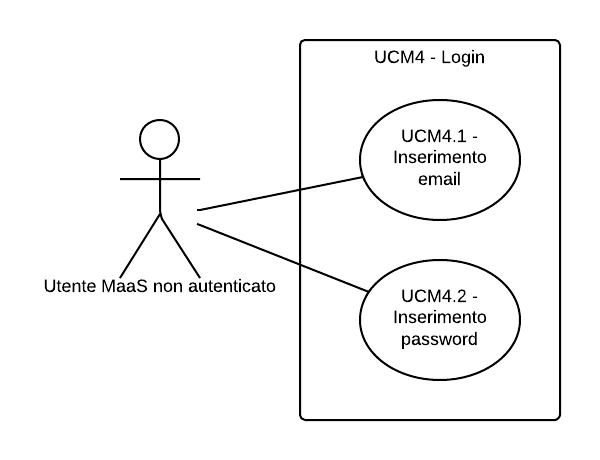
\includegraphics[scale=0.16]{UML/UCM4 - Login.png}
      \caption{UCM4 - Login}
      \end{center} 
    \end{figure}  
    
      %Tabella 
      \begin{center}
      \bgroup
      \def\arraystretch{1.8}     
      \begin{longtable}{  p{3.5cm} | p{8cm} } 
            
      \hline
      \multicolumn{2}{ | c | }{ \cellcolor[gray]{0.9} \textbf{UCM4 - Login}} \\ 
      \hline
      
      \textbf{Attori Primari} & Utente MaaS non autenticato \\ 
          \textbf{Scopo e Descrizione} & L'utente \glossario{MaaS} non autenticato intende accedere al servizio e per farlo deve inserire le proprie credenziali. \\ 
          
          \textbf{Precondizioni}  & Il servizio \glossario{MaaS} è pronto ed attende il login dell'utente.\\ 
          
          \textbf{Postcondizioni} & Il servizio \glossario{Maas} ha verificato le credenziali utente ed ha eseguito l'autenticazione di quest'ultimo. \\
          \textbf{Flusso Principale} & 1. L'utente inserisce l'email (UCM4.1); \newline
2. L'utente inserisce la password (UCM4.2). \\
           \textbf{Scenari Alternativi} & 1. L'utente non autenticato non effettua il login lasciando la pagina. \\
      \end{longtable}
      \egroup
\end{center}

\subsubsection{UCM5 - Credenziali errate} 
      %Tabella 
      \begin{center}
      \bgroup
      \def\arraystretch{1.8}     
      \begin{longtable}{  p{3.5cm} | p{8cm} } 
            
      \hline
      \multicolumn{2}{ | c | }{ \cellcolor[gray]{0.9} \textbf{UCM5 - Credenziali errate}} \\ 
      \hline
      
      \textbf{Attori Primari} & Utente MaaS non Autenticato \\ 
          \textbf{Scopo e Descrizione} & L'utente visualizza un messaggio di errore dato dall'inserimento di credenziali errate. \\ 
          
          \textbf{Precondizioni}  & Il sistema \glossario{MaaS} verifica le credenziali che l'utente ha inserito.\\ 
          
          \textbf{Postcondizioni} & Il sistema \glossario{MaaS} visualizza all'utente un messaggio di errore dopo aver verificato e non accettato le credenziali inserite. \\
      \end{longtable}
      \egroup
\end{center}

\subsubsection{UCM6 - Modifica profilo} 
    \begin{figure}[H]
      \begin{center}
      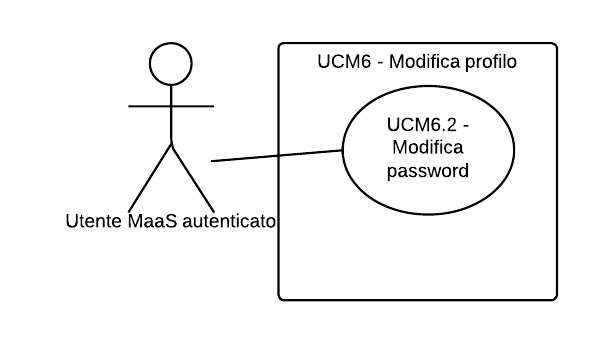
\includegraphics[scale=0.16]{UML/UCM6 - Modifica profilo.png}
      \caption{UCM6 - Modifica profilo}
      \end{center} 
    \end{figure}  
    
      %Tabella 
      \begin{center}
      \bgroup
      \def\arraystretch{1.8}     
      \begin{longtable}{  p{3.5cm} | p{8cm} } 
            
      \hline
      \multicolumn{2}{ | c | }{ \cellcolor[gray]{0.9} \textbf{UCM6 - Modifica profilo}} \\ 
      \hline
      
      \textbf{Attori Primari} & Utente MaaS autenticato \\ 
          \textbf{Scopo e Descrizione} & L'utente autenticato nel servizio può modificare la propria password. \\ 
          
          \textbf{Precondizioni}  & Il sistema è pronto, visualizza la pagina per la modifica del profilo utente e attende che l'utente interagisca.\\ 
          
          \textbf{Postcondizioni} & Il sistema \glossario{MaaS} ha acquisito le informazioni inserite dall'utente ed ha effettuato le modifiche. \\
          \textbf{Flusso Principale} & 1. L'utente \glossario{MaaS} autenticato può modificare la password (UCU6.1). \\
           \textbf{Scenari Alternativi} & L'utente può non modificare i propri dati lasciandoli invariati uscendo dalla pagina. \\
      \end{longtable}
      \egroup
\end{center}

\subsubsection{UCM6.1 - Modifica password} 
      %Tabella 
      \begin{center}
      \bgroup
      \def\arraystretch{1.8}     
      \begin{longtable}{  p{3.5cm} | p{8cm} } 
            
      \hline
      \multicolumn{2}{ | c | }{ \cellcolor[gray]{0.9} \textbf{UCM6.1 - Modifica password}} \\ 
      \hline
      
      \textbf{Attori Primari} & Utente MaaS autenticato \\ 
          \textbf{Scopo e Descrizione} & L'utente intende modificare la password di accesso al servizio. \\ 
          
          \textbf{Precondizioni}  & Il sistema predispone della pagina di modifica profilo ed attende che l'utente modifichi la password.\\ 
          
          \textbf{Postcondizioni} & \glossario{MaaS} ha memorizzato l'informazione datagli dall'utente. \\
      \end{longtable}
      \egroup
\end{center}

\subsubsection{UCM7 - Eliminazione account} 
      %Tabella 
      \begin{center}
      \bgroup
      \def\arraystretch{1.8}     
      \begin{longtable}{  p{3.5cm} | p{8cm} } 
            
      \hline
      \multicolumn{2}{ | c | }{ \cellcolor[gray]{0.9} \textbf{UCM7 - Eliminazione account}} \\ 
      \hline
      
      \textbf{Attori Primari} & Utente MaaS Autenticato \\ 
          \textbf{Scopo e Descrizione} & L'utente accede alla propria pagina profilo nella quale è presente un'azione che gli permette di eliminare il suo account. \\ 
          
          \textbf{Precondizioni}  & Il sistema \glossario{MaaS} ha predisposto una apposita azione per eliminare l'account dell'utente.\\ 
          
          \textbf{Postcondizioni} & Il sistema \glossario{MaaS} ha eliminato l'account dell'utente. \\
      \end{longtable}
      \egroup
\end{center}

\subsubsection{UCM8 - Gestione file di configurazione} 
    \begin{figure}[H]
      \begin{center}
      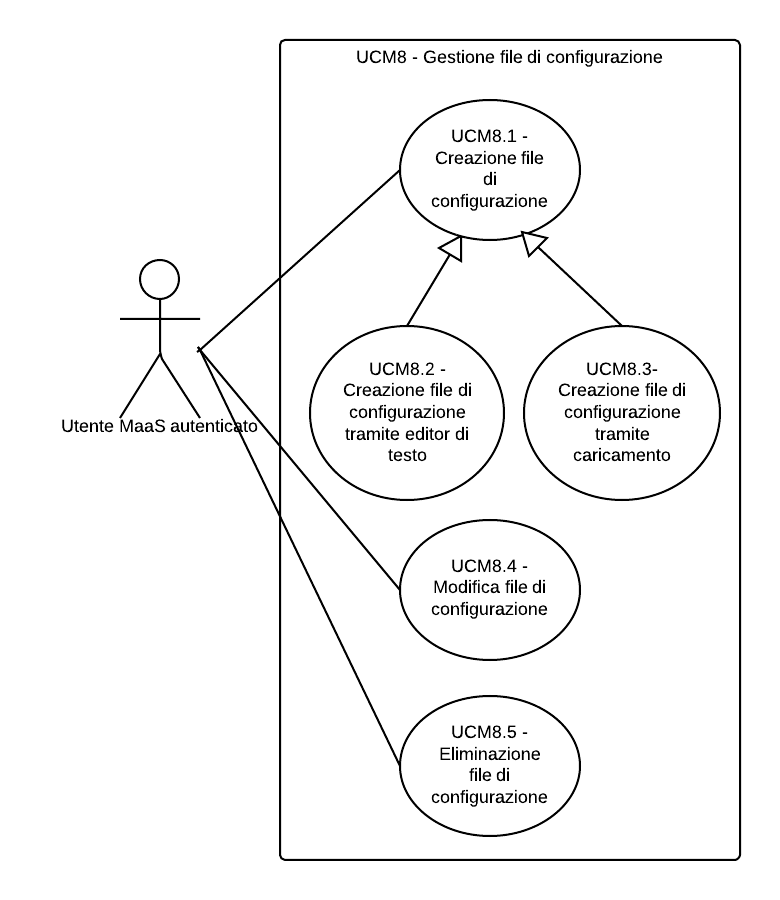
\includegraphics[scale=0.16]{UML/UCM8 - Gestione file di configurazione.png}
      \caption{UCM8 - Gestione file di configurazione}
      \end{center} 
    \end{figure}  
    
      %Tabella 
      \begin{center}
      \bgroup
      \def\arraystretch{1.8}     
      \begin{longtable}{  p{3.5cm} | p{8cm} } 
            
      \hline
      \multicolumn{2}{ | c | }{ \cellcolor[gray]{0.9} \textbf{UCM8 - Gestione file di configurazione}} \\ 
      \hline
      
      \textbf{Attori Primari} & Utente MaaS Autenticato \\ 
          \textbf{Scopo e Descrizione} & L'utente può gestire i file di configurazione attraverso i quali può registrare una nuova \glossario{Collection} e specificare la connessione al database delle \glossario{Collection} e/o al database delle credenziali. \\ 
          
          \textbf{Precondizioni}  & Il sistema \glossario{MaaS} visualizza la pagina necessaria alla gestione dei file di configurazione.\\ 
          
          \textbf{Postcondizioni} & Il sistema \glossario{MaaS} ha eseguito le azioni di configurazione dell'utente. \\
          \textbf{Flusso Principale} & 1. L'utente \glossario{MaaS} autenticato può creare file di configurazione (UCM8.1) in due modalità:  \newline
     L'utente \glossario{MaaS} autenticato può creare file di configurazione tramite editor di testo (UCM8.2); \newline
     L'utente \glossario{MaaS} autenticato può creare file di configurazione tramite caricamento (UCM8.3); \newline
2. L'utente \glossario{MaaS} autenticato dopo la creazione del file di configurazione lo può modificare (UCM8.4); \newline
3. L'utente \glossario{MaaS} autenticato può eliminare un file di configurazione (UCM8.5). \\
          
      \end{longtable}
      \egroup
\end{center}

\subsubsection{UCM8.1 - Creazione file di configurazione} 
      %Tabella 
      \begin{center}
      \bgroup
      \def\arraystretch{1.8}     
      \begin{longtable}{  p{3.5cm} | p{8cm} } 
            
      \hline
      \multicolumn{2}{ | c | }{ \cellcolor[gray]{0.9} \textbf{UCM8.1 - Creazione file di configurazione}} \\ 
      \hline
      
      \textbf{Attori Primari} & Utente MaaS Autenticato \\ 
          \textbf{Scopo e Descrizione} & L'utente ha la possibilità di creare il file di configurazione tramite editor di testo o di caricarlo tramite caricamento. \\ 
          
          \textbf{Precondizioni}  & Il sistema \glossario{MaaS} visualizza la pagina necessaria alla creazione o al caricamento dei file di configurazione.\\ 
          
          \textbf{Postcondizioni} & Il sistema \glossario{MaaS} ha eseguito correttamente la creazione del file di configurazione. \\
      \end{longtable}
      \egroup
\end{center}

\subsubsection{UCM8.2 - Creazione file di configurazione tramite editor di testo} 
      %Tabella 
      \begin{center}
      \bgroup
      \def\arraystretch{1.8}     
      \begin{longtable}{  p{3.5cm} | p{8cm} } 
            
      \hline
      \multicolumn{2}{ | c | }{ \cellcolor[gray]{0.9} \textbf{UCM8.2 - Creazione file di configurazione tramite editor di testo}} \\ 
      \hline
      
      \textbf{Attori Primari} & Utente MaaS Autenticato \\ 
          \textbf{Scopo e Descrizione} & L'utente visualizza un editor di testo con il quale può effettuare la creazione dei file di configurazione.
Tale editor sarà visualizzato come una text area nella pagina. \\ 
          
          \textbf{Precondizioni}  & Il sistema \glossario{MaaS} fornisce un editor di testo per la creazione dei file di configurazione.\\ 
          
          \textbf{Postcondizioni} & Il sistema \glossario{MaaS} fornisce un editor di testo per la creazione dei file di configurazione. \\
      \end{longtable}
      \egroup
\end{center}

\subsubsection{UCM8.3 - Creazione file di configurazione tramite caricamento} 
      %Tabella 
      \begin{center}
      \bgroup
      \def\arraystretch{1.8}     
      \begin{longtable}{  p{3.5cm} | p{8cm} } 
            
      \hline
      \multicolumn{2}{ | c | }{ \cellcolor[gray]{0.9} \textbf{UCM8.3 - Creazione file di configurazione tramite caricamento}} \\ 
      \hline
      
      \textbf{Attori Primari} & Utente MaaS Autenticato \\ 
          \textbf{Scopo e Descrizione} & L'utente può caricare il proprio file di configurazione. \\ 
          
          \textbf{Precondizioni}  & Il sistema \glossario{MaaS} fornisce un sistema di caricamento per i file di configurazione.\\ 
          
          \textbf{Postcondizioni} & Il sistema \glossario{MaaS} carica correttamente il file di configurazione \\
      \end{longtable}
      \egroup
\end{center}

\subsubsection{UCM8.4 - Modifica file di configurazione} 
      %Tabella 
      \begin{center}
      \bgroup
      \def\arraystretch{1.8}     
      \begin{longtable}{  p{3.5cm} | p{8cm} } 
            
      \hline
      \multicolumn{2}{ | c | }{ \cellcolor[gray]{0.9} \textbf{UCM8.4 - Modifica file di configurazione}} \\ 
      \hline
      
      \textbf{Attori Primari} & Utente MaaS Autenticato \\ 
          \textbf{Scopo e Descrizione} & L'utente dopo aver scelto il file di configurazione può modificarlo tramite editor di testo. \\ 
          
          \textbf{Precondizioni}  & Il sistema \glossario{MaaP} visualizza il file scelto dall'utente ed è pronto per la modifica.\\ 
          
          \textbf{Postcondizioni} & Il sistema \glossario{MaaP} esegue correttamente la modifica del file e lo salva. \\
      \end{longtable}
      \egroup
\end{center}

\subsubsection{UCM8.5 - Eliminazione file di configurazione} 
      %Tabella 
      \begin{center}
      \bgroup
      \def\arraystretch{1.8}     
      \begin{longtable}{  p{3.5cm} | p{8cm} } 
            
      \hline
      \multicolumn{2}{ | c | }{ \cellcolor[gray]{0.9} \textbf{UCM8.5 - Eliminazione file di configurazione}} \\ 
      \hline
      
      \textbf{Attori Primari} & Utente MaaS Autenticato \\ 
          \textbf{Scopo e Descrizione} & L'utente può eliminare il file di configurazione scelto. \\ 
          
          \textbf{Precondizioni}  & Il sistema \glossario{MaaS} ha predisposto per ogni file di configurazione la possibilità di eliminarlo.\\ 
          
          \textbf{Postcondizioni} & Il sistema \glossario{MaaS} ha eliminato correttamente il file di configurazione. \\
      \end{longtable}
      \egroup
\end{center}
